\documentclass[a4paper,12pt]{article}

\usepackage[T1]{fontenc}
\usepackage{xltxtra}
\usepackage[francais]{babel}
\usepackage{fancyhdr}

\usepackage{epsfig}
\usepackage{calc}
\usepackage{url}
\usepackage{boxedminipage}

\usepackage{titlesec}
%Pour enlever cette merde de chapter!
%\titleformat{\chapter}[hang]{\bf\huge}{\thechapter}{2pc}{}
\usepackage{graphicx}
%\usepackage{svg}
\usepackage{xcolor}
\usepackage{float}

\usepackage{tabularx}
\usepackage[colorlinks=true, linkcolor=black, citecolor=violet, urlcolor=blue]{hyperref}
\usepackage[sort, authoryear]{natbib}
\usepackage{subcaption}
\bibpunct{[}{]}{,}{n}{,}{,}

% --------------------------------
%Pour compiler sur Manjaro        
\usepackage[utf8]{inputenc}
\usepackage{algorithmicx}
\usepackage{algpseudocode}
% --------------------------------
%Pour les tableaux multi-colonnes
\usepackage{multirow}

\setcounter{page}{1}
\pagenumbering{Roman}
%%\onehalfspacing

%%%%%%%%%%%%%%%%%%%%%%%%%%%%%%%%%%%%%%%%%%%%%%%%%%%%%%%%%%%
%%%%%%%%%%%%%%%%%%%%%%%%%%%%%%%%%%%%%%%%%%%%%%%%%%%%%%%%%%%
%% Définitions à personnaliser 

%% Pour les noms, utilisez la première lettre du prénom suivi du 
%% nom de famille (première lettre majuscule, reste en minuscule).


%%%% Indiquer le nom de l'encadrant ci-dessous:

\def\nomEncad{Martin \textsc{Quinson}}

%% Si le projet est co-encadré indiquer les deux noms à la suite dans 
%% Le même champs


%%%% Indiquer les noms des étudiants participant ci-dessous:

\def\nomEtudA{Louisa \textsc{Bessad}}

%% Si le projet est encadré par moins de 4 étudiants laissez
%% les variables inutiles vides


%%%% Indiquer la référence (numero) et le nom du sujet ci-dessous:

\def\refProjet{Numéro Projet} 
\def\titreProjetCourt{Titre court}
\def\titreProjetLong{Real-time online emulation of real applications on SimGrid with Simterpose}

%% Le titre court ne doit pas faire plus d'une vingtaine de caractère
%% résumez le à quelques mots essenciels


%%%% Indiquer le type de document et sa version ci-dessous:

\def\typeDoc{Pré-rapport}
 
%% - Rapport intermédaire
%% - Rapport final

%\let\origsec\section
%\renewcommand{\section}[1]{\newpage\origsec{#1}}



%%%%%%%%%%%%%%%%%%%%%%%%%%%%%%%%%%%%%%%%%%%%%%%%%%%%%%%%%%%
%%%%%%%%%%%%%%%%%%%%%%%%%%%%%%%%%%%%%%%%%%%%%%%%%%%%%%%%%%%
%% Définitions à ne pas modifier
 
%%%% ||| Mise en page verticale ||| 
\setlength{\voffset}{-1in} % a4:reste 297mm pour les 5 suivants:
\setlength{\topmargin}{15mm}         % avant l'en-tête
\setlength{\headheight}{20mm}        % hauteur de l'en-tête 
\setlength{\headsep}{10mm}            % entre l'en-tête et le corps
\setlength{\textheight}{220mm}       % hauteur du corps
\setlength{\footskip}{12mm}          % pied de page par rapport au corps 
%\setlength{\footlength}{2em}

%%%%% --- Mise en page horizontale ---
\setlength{\hoffset}{-1in} % a4:reste 210mm 
\setlength{\oddsidemargin}{25mm}     % entre hoffset et le corps
\setlength{\evensidemargin}{25mm}    % entre hoffset et le corps
\setlength{\marginparwidth}{0mm}     % largeur de la marge
\setlength{\marginparsep}{0mm}       % séparateur corps marge
\setlength{\textwidth}{160mm}        % largeur du corps

%\usepackage{fullpage}
%\setlength{\headheight}{20mm}        % hauteur de l'en-tête 
%\setlength{\headsep}{10mm}            % entre l'en-tête et le corps
%\setlength{\textheight}{200mm}
%\setlength{\footskip}{0mm}          % pied de page par rapport au corps 

\def\annee{2015}



%%%%%%%%%%%%%%%%%%%%%%%%%%%%%%%%%%%%%%%%%%%%%%%%%%%%%%%%%%%
%% Début du document

\begin{document}
\begin{titlepage}

\newcommand{\HRule}{\rule{\linewidth}{0.5mm}} % Defines a new command for the horizontal lines, change thickness here

\center % Center everything on the page
 
%----------------------------------------------------------------------------------------
%	HEADING SECTIONS
%----------------------------------------------------------------------------------------

\textsc{\LARGE Université Pierre et MArie Curie}\\[0.44cm] % Name of your university/college
\textsc{\Large Master informatiqe}\\[0.44cm] % Major heading such as course name
\textsc{\large Systèmes et Applications Répartis}\\[1.44cm] % Minor heading such as course title

\textsc{\LARGE Loria}\\[0.44cm] % Name of your university/college
\textsc{\Large Equipe VERIDIS}\\[1.44cm] % Major heading such as course name

%----------------------------------------------------------------------------------------
%	TITLE SECTION
%----------------------------------------------------------------------------------------

\HRule \\[0.4cm]
{ \huge \bfseries Real-time online emulation of real applications on SimGrid with Simterpose}\\[0.4cm] % Title of your document
\HRule \\[1.44cm]
 
%----------------------------------------------------------------------------------------
%	AUTHOR SECTION
%----------------------------------------------------------------------------------------

\begin{minipage}{0.4\textwidth}
\begin{flushleft} \large
\emph{Etudiant:}\\
Louisa \textsc{Bessad} % Your name
\end{flushleft}
\end{minipage}
~
\begin{minipage}{0.4\textwidth}
\begin{flushright} \large
\emph{Encadrant} \\
Martin \textsc{Quinson} % Supervisor's Name
\\\vspace{1.44cm} \emph{Rapporteur:} \\ Sébastien
\textsc{Monnet}
\end{flushright}
\end{minipage}\\[1.5cm]

% If you don't want a supervisor, uncomment the two lines below and remove the section above
%\Large \emph{Author:}\\
%John \textsc{Smith}\\[3cm] % Your name

%----------------------------------------------------------------------------------------
%	DATE SECTION
%----------------------------------------------------------------------------------------

{\large \today}\\[1.5cm] % Date, change the \today to a set date if you want to be precise

%----------------------------------------------------------------------------------------
%	LOGO SECTION
%----------------------------------------------------------------------------------------

%\includegraphics{Logo}\\[1cm] % Include a department/university logo - this will require the graphicx package
\includegraphics[scale=0.2]{Pictures/png/UPMC_sorbonne.png}\hspace{3cm}
\includegraphics[scale=0.1]{Pictures/loria_logo.jpg}

%----------------------------------------------------------------------------------------

\vfill % Fill the rest of the page with whitespace
\end{titlepage}
\clearpage
%\vfill

%%\newpage
%%\mbox{}
%%\newpage

%%%%%%%%%%%%%%%%%%%%%%%%%%%%%%%%%%%%%%%%%%%%%%%%%%%%%%%%%%%
%% Définition des en-têtes et pied de pages
\pagestyle{fancyplain}
%\fancyhead{}
%\fancyfoot{}
%
\fancyhead[L]{\textsc{Université Pierre et Marie Curie} \\ {\color{white} b} \\ \nomEtudA}
\fancyhead[C]{\textbf{Pré-rapport}}%\\\titreProjetCourt}}
\fancyhead[R]{\textsc{LORIA} \\ {\color{white} b} \\ \nomEncad}

\fancyfoot[L]{\includegraphics[width=3cm]{Pictures/png/UPMC_sorbonne.png}}
\fancyfoot[C]{\textbf{\thepage}}
\fancyfoot[R]{\includegraphics[width=4cm]{Pictures/loria_logo.jpg}}

%\lhead[\fancyplain{}{\texttt{Université Pierre et Marie Curie}\\
%          Master Informatique\\ UE \textbf{PSAR} fév. \annee \\ \nomEncad}]
%      {\fancyplain{}{\textsc{Université Pierre et Marie Curie}\\
%          Master Informatique\\ UE \textbf{PSAR} \annee \\ \nomEncad}}
%\chead[\fancyplain{}{\textbf{Projet \refProjet\\\titreProjetCourt}}]
%      {\fancyplain{}{\textbf{Projet \refProjet\\\titreProjetCourt}}}
%\rhead[\fancyplain{}{\nomEtudA\\\nomEtudB}]
%      {\fancyplain{}{\nomEtudA\\\nomEtudB}}
%\lfoot[\fancyplain{}{\epsfig{figure=UPMC_sorbonne.eps,width=3cm}}]
%      {\fancyplain{}{\epsfig{figure=UPMC_sorbonne.eps,width=3cm}}}
%\cfoot[\fancyplain{}{\textbf{\thepage/\pageref{fin}}}]
%      {\fancyplain{}{\textbf{\thepage/\pageref{fin}}}}
%\rfoot[\fancyplain{}{\typeDoc}]
%      {\fancyplain{}{\typeDoc}}


%%%%%%%%%%%%%%%%%%%%%%%%%%%%%%%%%%%%%%%%%%%%%%%%%%%%%%%%%%%


\tableofcontents
%\vfill
\newpage
%% \mbox{}
%% \newpage

\listoffigures
\newpage

\listoftables
\newpage
%% \mbox{}
%% \newpage

%Abstract
%\begin{abstract}
 %TODO
  %% Dans le cadre de ce stage nous allons nous intéresser aux applications ditribuées à large échelle et comment on peut les tester et évaluer leurs performances via une combinaison d'émulation et de simulation en utilisant SIMGRID et Simterpose qui sont deux projets européens. SIMGRID a été lancé en 1999 pour étudier des algorithmes d'ordonnancement sur des plateformes hétérogènes dans un environnement distribué et faciliter leur programmation. Il fournit les outils de base nécessaire à la simulation de ce type d'applications. Simterpose s'insère dans le projet SIMGRID afin de pouvoir étudier des applications complètes et pas uniquement leur modèle que l'on fournit habituellement en paramètre au simulateur. Le but est de faire de l'émulation en utilisant un simulateur que sera SIMGRID. Puisque nous nous intéressons aux applications distribuées notre émulateur doit pouvoir\textit{i)} exécuter un grand nombre d'instances d'une même application sur un même système afin de pouvoir debugguer, \textit{ii)} évaluer des applications ayant de nombreuses condition d'exécution (simple n\oe ud, réseau complet), \textit{iii)} collecter les informations concernant l'application pendant qu'elle s'exécute.
%\end{abstract}
%\newpage

{\color{white} blabla} \vspace{7cm}

Ce stage se déroule au Loria, Laboratoire Lorrain de Recherche en Informatique
et ses Applications, unité mixte de recherche commune à plusieurs
établissements: le CNRS, l'INRIA, et l' Université de Lorraine. Le LORIA a pour
mission la recherche fondamentale et appliquée en sciences informatiques et ce,
depuis sa création, en 1997.

L'encadrement est assuré par Martin Quinson au sein de l'équipe VERIDIS, dont les sujets de recherches sont la conception de méthodes pour les systèmes distribués et d'outils pour la vérification et la validation de systèmes.



\newpage

{\color{white} blabla} \vspace{7cm}


Je voudrais remercier mon tuteur Martin Quinson pour m'avoir permis d'effectuer ce stage, durant lequel j'ai beaucoup appris.

Je tiens également à remercier mon encadrant universitaire Sébastien Monnet pour ses précieux conseils.

\newpage

\setcounter{page}{1}
\pagenumbering{arabic}
% Content

\section{Introduction}

%% intro/objectif: virtualisation légère d'applications distribuées (tester des applications distribuées réelles: test regression et performance, légère car on veut tester des centaines d'instances)

%% Applications: stockage distribué (CEPH, TAHOE/LAFS) et RT event processing (Storm)

Dans le cadre de ce stage, nous allons nous intéresser aux applications distribuées. \textit{ Autrement dit aux} applications dont une partie ou la totalité des ressources  n'est pas stockée sur la machine où l'application s'exécute, mais sur plusieurs machines distinctes. Ces dernières communiquent entre elles via le réseau pour s'échanger les données nécessaires à l'exécution de l'application. Les applications distribuées ont de nombreux avantages; elles permettent notamment d'augmenter la disponibilités des données en se les échangeant,\textit{ comme les applications Torrent (BitTorrent, $µ$Torrent...)}. Grâce au projet BOINC\footnote{\url{https://boinc.berkeley.edu/}} par exemple, on peut partager la puissance de calcul inutilisée de sa machine. Depuis une dizaine d'années la popularité de ces applications distribuées ne cesse de croître. Elles deviennent de plus en plus complexes avec des contraintes et des exigences de plus en plus fortes, en particulier au niveau des performances et de l'hétérogénéité des plate-formes et des ressources utilisées. Il devient donc de plus en plus difficiles de créer de telles applications mais aussi de les tester. En effet, malgré l'évolution des applications distribuées, les protocoles d'évaluation de leurs performances n'ont que peu évolués.

Actuellement, il existe trois façons de tester le comportement d'applications distribuées; l'exécution sur plate-forme réelle, la simulation et l'émulation. 

La première solution consiste à exécuter réellement l'application sur un parc de machines et d'étudier son comportement en temps-réel. Cela permet de la tester sur un grand nombre d'environnement. L'outil créé et développé en partie en France pour nous permettre de faire cela est \textbf{Grid'5000}\footnote{Infrastructure de 8000 c\oe urs répartis dans la France entière crée en 2005. \\ \url{https://www.grid5000.fr/mediawiki/index.php/Grid5000:Home}}\citet{GRID5000}, un autre outil développé à l'échelle mondiale est \textbf{PlanetLab} \footnote{Crée en 2002, cette infrastructure de test compte aujourd'hui 1340 noeuds. \\ \url{http://www.planet-lab.org}}. Néanmoins pour mettre en \oe uvre ces solutions complexes, il faut disposer des infrastructures nécessaires pour effectuer les tests. Il faut également écrire une application capable de gérer toutes ces ressources disponibles. De plus, du fait du partage des différentes plate-formes entre plusieurs utilisateurs, les expériences ne sont pas forcément reproductibles. 

{\color{red}\textit{La seconde solution consiste à faire de la simulation, c'est-à-dire à utiliser un programme appelé simulateur pour nous permettre de simuler ce que l'on souhaite étudier.}} Dans notre cas, pour pouvoir tester des applications distribuées sur un simulateur, on doit d'abord représenter de façon théorique l'application ainsi que l'environnement d'exécution. Pour cela, on identifie les propriétés de l'application et de son environnement puis on les transforme à l'aide de modèles mathématiques. Ainsi, on va exécuter dans le simulateur le modèle de l'application dans un environnement également modélisé et non l'application réelle. Cette solution est donc facilement reproductible, simple à mettre en \oe uvre, \textit{ quand on sait} modéliser l'application, et permet de prédire l'évolution du système étudié grâce à l'utilisation de modèles mathématiques. De nos jours, les simulateurs, tel que  \textbf{SIMGRID}\citet{SIMULATIONCASANOVA, SIMULATIONMARTIN}, peuvent simuler des applications distribuées mettant à contribution des milliers de noeuds. Néanmoins, avec la simulation on ne peut valider qu'un modèle et pas l'application elle même puisqu'on exécute seulement un modèle. 

La troisième solution consiste à faire de l'émulation, cela signifie que nous allons exécuter réellement l'application mais dans un environnement virtualisé grâce à un logiciel, l'émulateur. Ce dernier joue le rôle d'intercepteur et utilise un simulateur pour virtualiser l'environnement d'exécution.
%On fera ainsi croire à l'application qu'elle s'exécute sur une machine autre que l'hôte.
Cette solution représente un intermédiaire entre la simulation et l'exécution sur plate-forme réelle visant à résoudre les limitations de ces deux solutions. En effet, les actions de l'application sont réellement exécutées sur la machine hôte, autrement dit la machine réelle sur laquelle s'exécute l'émulation. Mais on fait croire à l'application grâce au simulateur qu'elle se trouve dans un environnement différent de la machine \textit{réelle}. De plus, cela évite d'avoir deux versions de l'application en terme de code: une pour la simulation et une pour la production. Dans notre cas l'émulation peut-être faite \textit{off-line}; on sauvegarde les actions de l'application sur disque et on les rejoue plus tard dans le simulateur ou \textit{on-line}; \textit{ on bloque l'application le temps que les actions soient reportées dans le simulateur pour qu'il calcule le temps de réponse de la plate-forme simulée}.

Dans le cadre du projet Simterpose c'est l'émulation qui a été choisie pour tester des applications distribuées. En effet la simulation n'était pas une bonne solution puisque nous voulons valider les applications et non leur modèle. En ce qui concerne l'exécution sur plate-forme réelle, il y avait trop de contraintes matérielles à satisfaire.

{\color{red}TODO: Transition}
Il existe deux types d'émulation pour les applications distribuées; la virtualisation standard et la ``légère''. On parle de virtualisation ``légère'' quand on souhaite tester des applications sur une centaine d'instances. Dans ce rapport nous allons présenter en section \ref{section:emulation} les méthodes utilisées pour faire de la virtualisation légère: limitation et interception. Puis en section \ref{section:sota} nous verrons les projets qui existent aujourd'hui pour ce type de virtualisation. Pour finir en section \ref{section:simterpose} nous expliquerons pourquoi dans le cadre du projet Simterpose c'est la virtualisation légère par interception qui a été choisie et comment elle fonctionne.

\newpage
\section{Méthodes possibles pour la virtualisation légère}
\subsection{Emulation par limitation / Virtualisationi standard}
\begin{itemize}
\item principe: limiter l'accès aux ressources par exemple (cgroup, netstat, cpuburner), temps d'un SEB (bench avec netlink, limiter (cap))
\item avantage plus simple
\item désavantages: host>>target, modèle à vérifier, contrôle expérimental fin
\end{itemize}

\subsection{Emulation par interception}
 principe: interception des actions et médiation (pas juste intereption et rejeu). Intercepter des symbôles pour en changer l'effet

\subsubsection{Action sur le fichier source}
reimplem SMPI ( trop spé) ,source to source/ pass LLVM( gcc+libc=consanguin) 

\subsubsection{Action sur le binaire}
Valgrind (perf pourrie)

\subsubsection{Médiation directe des appels de fonctions}
pourquoi: pthread, temps

\paragraph{linker: LD\_PRELOAD}
pas suid
%% On pourrait alors penser qu'une bonne solution serait d'intercepter les actions
%% de l'application au niveau des bibliothèques.{\color{red} rajouter des trucs sur
%%   VDSO}. Pour cela il existe la variable d'environnement \textbf{LD\_PRELOAD}
%% qui contient la liste des bibliothèques à précharger et qui est utilisée par le
%% noyau lors du premier lancement d'un programme. En effet par défaut Linux
%% effectue une édition de lien dynamiqe, l'édition de lien statique n'étant
%% choisie qu'en l'absence de bibliothèques partagées définissant les fonctions
%% utilisées par l'application. On va donc créer notre propre bibliothèque de
%% fonctions surchargeant chaque fonction susceptible d'être utilisée par
%% l'application. Une fonction surchargée contiendra alors toutes les modifications
%% nécessaires pour maintenir notre environnement simulé suivi de l'appel à la
%% fonction initiale puisqu'on souhaite juste intercepter l'appel et pas
%% l'empêcher. On préchargera cette bibliothèque avant les autres en la plaçant
%% dans la variable LD\_PRELOAD, ainsi nos fonctions passeront avant les fonctions
%% des bibliothèques usuelles.

%% Néanmoins si l'application fait un appel système directement sans passer par la
%% couche \textit{Bibliothèques} Fig.~\ref{AS_Communication} notre mécanisme
%% d'interception est countournée. En effet on ne peut surcharger que des fonctions
%% avec cette solution, pas des appels sytèmes. De même si on oublie de réécrire
%% une fonction d'une des bibliothèques utilisée par l'application. Cette solution
%% n'est donc pas suffisante pour le modèle d'interception que nous souhaitons
%% avoir.

%% Cependant on peut voir que LD\_PRELOAD résout les problèmes de ptrace concernant
%% les fonctions de temps, et inversement puisque ptrace permet d'intercepter les
%% appels systèmes que le modèle d'interception avec LD\_PRELOAD ne permet pas de
%% gérer. Une solution choisie lors d'un précédent stage est donc d'allier les
%% deux. On surchargera les fonctions temporelles dans notre bibliothèque
%% préchargée avec LD\_PRELOAD pour pallier les lacunes temporelles de ptrace. Et
%% pour toutes les autres fonctions ptrace s'en occupera, ainsi on est certain de
%% n'oublier aucune fonction. Maintenant que nous savons ce que nous devons
%% intercepter et comment l'intercepter nous allons voir ce que nous devons
%% modifier pour pouvoir maintenit notre émulation simulation.

%% \textit{Pour faire face à ce problème il a été choisi d'utiliser l'éditeur de
%%   lien dynamique \textbf{LD\_PRELOAD}, ce dernier intercepte les appels de
%%   l'application au niveau des bibliothèques. Pour cela on va créer une
%%   bibliothèque.}

\paragraph{linker got injection}
plus dur que nécessaire

\subsubsection{Médiation des Appels Système}
pourquoi: read/write, comm reseau

\paragraph{ptrace}
%% Nous allons intercepter les actions que sont les appels systèmes faits par
%% l'applciation, ainsi nous sommes sûrs d'intercepter tous les types de
%% communications que l'application est susceptible d'initier avec le noyau. Les
%% appels systèmes sont constitués de deux parties; la première, l'entrée,
%% initialise l'appel via les registres de l'application qui contiennent les
%% arguments de l'appel puis donne la main au noyau. La seconde, la sortie, inscrit
%% le retour de l'appel système dans le registre de retour de l'application, les
%% registres d'arguments contennant toujours les valeurs reçues à l'entrée de
%% l'appel système, et rend la main à l'application. Nous devons donc intercepter
%% les deux parties de l'appel système pour maintenir notre environnement simulé et
%% donc stopper l'application à chaque fois pour récupérer ou modifier les
%% informations nécéssaires avant de lui rendre la main pour entrer ou sortir de
%% l'appel système.

%% Pour faire cela il existe de nombreux outils de différents types. Il y a l'API
%% ptrace, qui est lui même un appel système et qui permet de tracer tous les
%% événement désirés d'un processus contrôlé. Néanmoins ce dernier fait de nombreux
%% changements de contexte pour intercepter des événements. De plus il gère mal les
%% processus quand on a du multithreading, et il ne fait pas parti de la norme
%% POSIX donc son exécution peut varier d'une machine à une autre. On trouve
%% ensuite les API noyau aussi appelées modules d'instrumentations telles que:
%% utrace, kprobes, uprobes{\color{red}citation}. Utrace fait la même chose que
%% ptrace mais en mode noyau. Cela permet d'éviter les nombreux changements de
%% contexte pour gérer l'appel système et que le noyau l'exécute {\color{green}
%%   clair?}. De plus il gère les événements de thread et non de processus comme
%% ptrace ce qui évite le problème de gestion du multhreading. Kprobes quant à lui
%% permet à un utilisateur d’insérer dynamiquement des points d'arrêts à des
%% endroits spécifiques du noyau, dans notre cas ce serait le code des appels
%% systèmes. Ainsi l’utilisateur peut fournir un handler particulier à exécuter
%% avant ou après l’instruction marquée. Quand un point d'arrêt est touché kprobe
%% prend la main et exécute le bon handler. Uprobes fait la même chose que kprobes
%% mais pour le code d'applications et pas le code du noyau. Ainsi pour chaque
%% point d'arrêt géré par uprobes on doit créer un module noyau qui contient le
%% handler à exécuter quand le point d'arrêt est atteint. Uprobes utilise utrace
%% pour savoir quand on atteint ou non un point d'arrêt. Les deux avantages des API
%% noyau est qu'elles sont rapides et qu'elles ont accès à toutes les ressources
%% sans aucune restriction, mais ce dernier point représente aussi leur plus gros
%% défaut de par sa dangerosité. De plus, dans notre cas il ne semble pas judicieux
%% de modifier le code du noyau ou de faire de la programmation noyau via des
%% modules dont il faudra également gérer le bon chargement. Malgrè ses défauts
%% c'est donc l'appel système ptrace qui a été choisi. Maintenant que nous savons
%% pourquoi nous allons utiliser ptrace comme intercepteur pour les appels systèmes
%% nous allons étudier son fonctionnement.

%% Pour intercepter les éventuels appels systèmes d'une applciation nous allons
%% donc utiliser l'appel système \textbf{ptrace}{\color{red}citation}. Il permet de
%% controler l'exécution de processus mais également d'écrire et de lire
%% directement dans l'espace d'adressage d'un processus. Pour cela on créé deux
%% processus; un qui exécutera l'application et qu'on souhaite contrôler, on
%% l'appellera ``processus espionné'' et un autre qui le contrôlera appelé
%% ``processus espion''. Le processus espionné indiquera au processus espion qu'il
%% souhaite être contrôlé via un appel système ptrace. À la reception de cet appel
%% le processus espion notifiera son attachement au processus espionné via un autre
%% appel à ptrace. Il indiquera également sur quelles actions du processus espionné
%% il veut être notifié, définissant ainsi les actions bloquantes pour le processus
%% espionné. Dans notre cas, ce seront les appels systèmes que l'on considérera
%% comme point d'arrêt pour le processus espionné. Ainsi quand un des processus de
%% l'application voudra faire un appel système quelconque il sera bloqué avant de
%% l'exécuter, l'appel système ptrace sera lancé et notifiera le processus
%% espion. Ce dernier fera les modifications nécessaires dans les registres du
%% processus espionné pour conserver la virtualisation de l'environnement, puis il
%% rendra la main au processus espionné bloqué pour que l'appel système puisse
%% avoir lieu. Au retour de l'appel système le processus espionné sera de noveau
%% stoppé, un ptrace sera envoye au processus espion qui remodifiera les
%% informations nécessaires. Puis il rendra la main au processus espionné bloqué
%% qui sortira de son appel système avec un résultat exécuté sur la machine hôte et
%% un temps d'exécution et une horloge fournie par le simulateur.

%% {\color{red} Mettre un schema attachement attente pere attrape signal modification main fils as retour pere...}

%% {\color{red} \textbf{gérer cette transition}} Néanmoins il a été montré dans un
%% précédent stage que l'appel système ptrace est inefficace voir inutile en ce qui
%% concerne tous les appels systèmes temporels qu'une application voudrait
%% faire. \textit{les appels systèmes ``time'', ``clock\_gettime'',
%%   ``gettimeofday'' avec \textbf{ptrace} ne sont pas possibles, d'où l'alliance
%%   avec LD\_PRELOAD} Par exemple lors d'un gettimeofday l'appel système n'est pas
%% lancé on répond directement au niveau de la bibliothèque ainsi on n'arrive même
%% pas au niveau de l'appel système, donc ptrace ne fait rien.  Problème
%% portabilité {\color{red} \textbf{gérer cette transition}}
\paragraph{uprobe}
Non module noyau

\paragraph{seqcomp/bpf}
Read only

\subsection{Émulation par limitation}
\label{section:limitation}
%% \begin{itemize}
%% \item principe: limiter l'accès aux ressources par exemple (cgroup, netstat, cpuburner), temps d'un SEB (bench avec netlink, limiter (cap))
%% \item avantage plus simple
%% \item désavantages: host>>target, modèle à vérifier, contrôle expérimental fin
%% \end{itemize}

Avec cette première méthode, illustrée Figure \ref{Virtu_limitation}, on place
la couche d'émulation au-dessus de la plateforme réelle (comme un hyperviseur
pour une VM). De fait, la puissance de l'émulateur dépend de la puissance de la
machine hôte et ne peux donc pas dépasser les capacités de cette dernière. De
plus, en choisissant de placer l'émulation comme une surcouche, cela permet de
limiter l'accès aux ressources pour les applications. En effet, elles ne
pourront pas passer la couche d'émulation pour accéder aux ressources localisées
sur la machine hôte. Les requêtes des applications seront arrêtées par
l'émulateur. C'est lui qui s'occupera de récupérer les ressources demandées par
les applications. Il existe différents outils permettant de mettre en place
cette virtualisation, on trouve notamment
\textbf{cgroups}\footnote{\url{https://www.kernel.org/doc/Documentation/cgroups/cgroups.txt}}
et \textbf{cpuburner} \citep{canon2006wrekavoc, buchert2011methods} pour le
système\footnote{\textbf{cgroups} contrôle que l'application ne reçoive pas plus
  de ressources que prévues, alors que \textbf{cpuburner} lance un programme
  glouton qui monopolise des ressources afin que l'application ne puisse
  utiliser que ce qu'on lui laisse.} et \textbf{iptables}\footnote{The netfilter.org project \url{http://www.netfilter.org/} \\ Man iptables \url{http://ipset.netfilter.org/iptables.man.html}} pour le réseau. L'émulation par
limitation a l'avantage d'être simple à mettre en \oe uvre puisque l'on se base
sur la machine hôte. Néanmoins, elle est assez contraignante du fait qu'on ne
puisse pas émuler des architectures plus performantes que l'hôte.

\begin{figure}[H]
  \centering
  \begin{subfigure}{0.4\textwidth}
    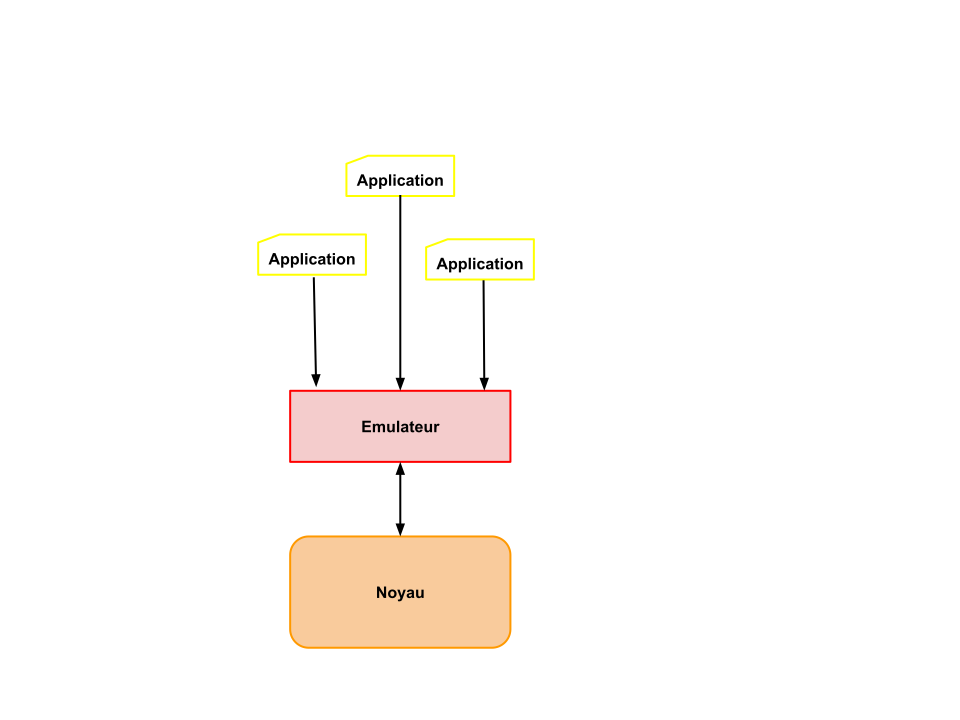
\includegraphics[scale=0.39]{Pictures/png/Virtualisation_limitation}
    \caption{Virtualisation par limitation}
    \label{Virtu_limitation}
  \end{subfigure}
  \begin{subfigure}{0.4\textwidth}
    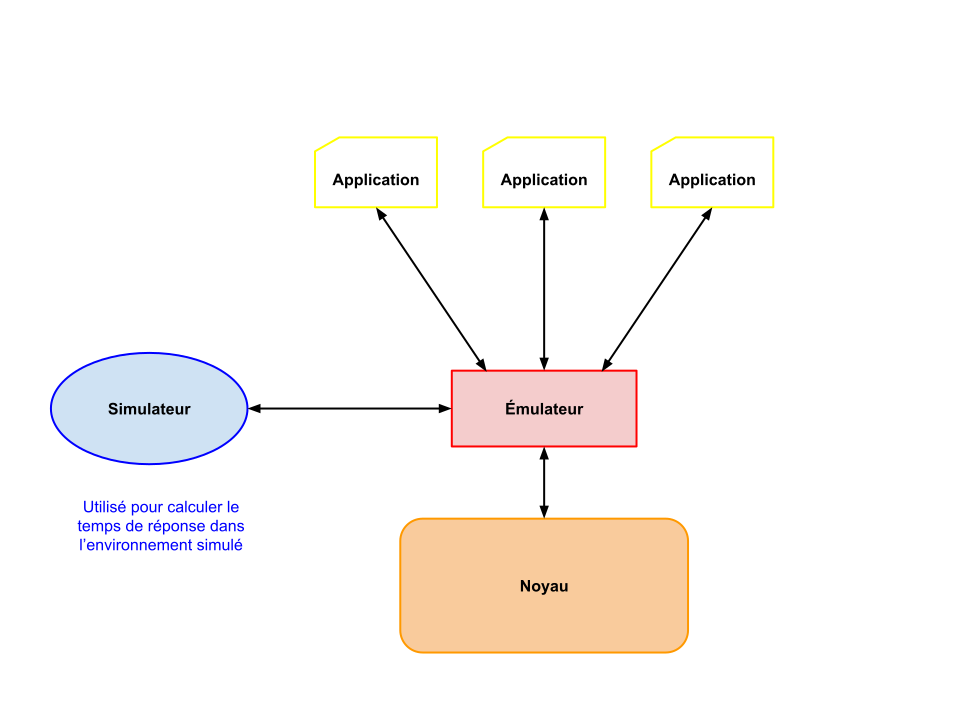
\includegraphics[scale=0.3]{Pictures/png/Virtualisation_interception}
    \caption{Virtualisation par interception}
    \label{Virtu_interception}
  \end{subfigure}
  \caption{Approches de virtualisation légère}
  \label{TYPE_VIRTUALISATION}
\end{figure}

\subsection{Emulation par interception}
\label{section:interception}
%% principe: interception des actions et médiation (pas juste interception et rejeu). Intercepter des symboles pour en changer l'effet

Dans le cas de l'émulation par interception, illustrée
Figure \ref{Virtu_interception} , pour mettre en place un environnement distribué
émulé sur lequel les applications penseront s'exécuter, deux outils vont être
utilisés; un simulateur pour virtualiser l'environnement d'exécution, et un
émulateur qui va intercepter toutes les communications de l'application avec l'hôte
et qui les transmettra ensuite au simulateur.

 \begin{figure}[H]
   \centering 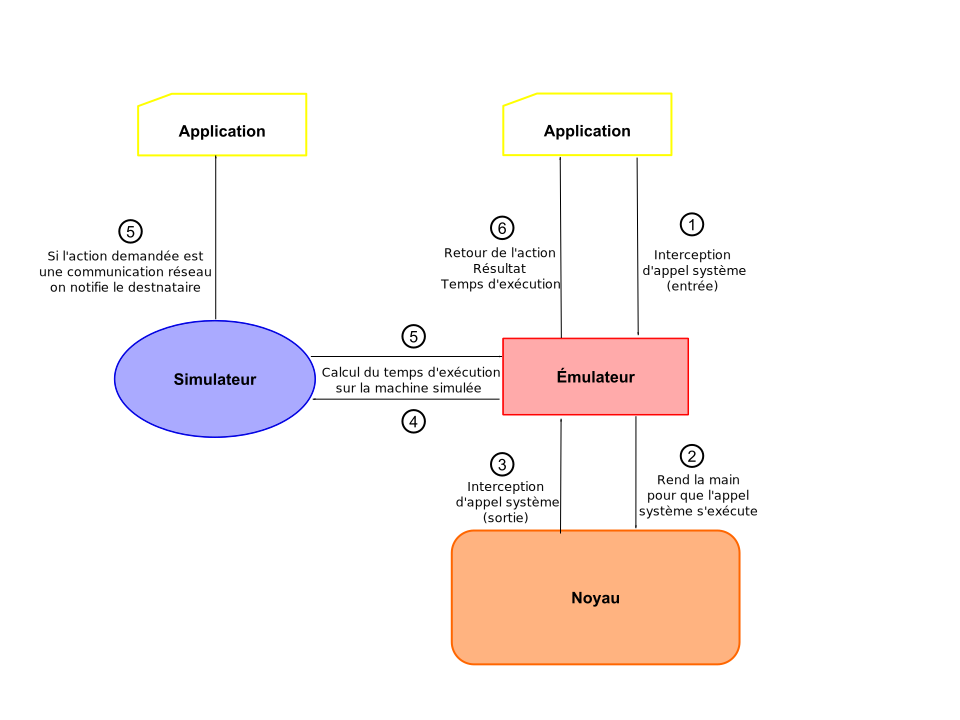
\includegraphics[scale=0.5]{Pictures/png/Emulation_fonctionnement}
   \caption{Fonctionnement de l'émulation par interception.}
   \label{INTERCEPTION}
 \end{figure}
 
 Une application distribuée peut vouloir interagir avec son environnement soit
 pour effectuer de simples calculs, soit pour effectuer des communications avec
 d'autres applications sur le réseau. Quand l'émulateur intercepte une
 communication venant d'un des processus d'une application, il modifie les
 caractéristiques de la communication pour qu'elle puisse s'exécuter sur la
 machine hôte. Il effectue l'opération inverse lorsque cette dernière envoie une réponse à
 l'application. En parallèle, l'émulateur demande au simulateur de calculer le
 temps d'exécution dans l'environnement virtuel de l'action
 demandée par l'application. L'émulateur renvoie ce temps à l'application en plus
 du résultat du calcul demandé pour mettre à jour son horloge. Ainsi, les
 calculs sont réellement exécutés sur la machine, les communications réellement
 émises sur le réseau géré par le simulateur et c'est le temps de réponse qu'il
 fourni qui va influencer l'horloge de l'application. Finalement, les
 applications ne communiquent plus directement entre elles.

\vspace{0.5cm}

\subsubsection{Action sur le fichier source}
\label{section:source}
%% reimplem SMPI (trop spé) ,source to source/ pass LLVM( gcc+libc=consanguin) 
%% , Coccinelle
Le premier niveau auquel on peut se placer pour intercepter les actions est le fichier source de l'application. On pourrait avant de compiler le code réécrire les parties qui nous intéressent.

Un premier outil pour cela est le programme Coccinelle \citep{cocci}. Il permet de trouver et transormer automatiquement des parties spécifiques d'un code source C. Pour cela, Coccinelle fournit le langage SmPL\footnote{Semantic Patch Language} permettant d'écrire les patchs sur lesquels il va se baser pour transformer le code. Un patch contient une suite de règles, chacune transforme le source en ajoutant ou supprimant du code. Lors de son exécution, Coccinelle scanne le code et cherche les lignes qui satisfont les conditions des règles spécifiées dans le patch et applique les transformations correspondantes. Dans notre cas, il s'agirait de toutes les actions de communications directes ou indirectes avec le noyau susceptibles de mettre à jour l'environnement virtuel. Néanmoins, il ne faut pas oublier de définir une règle pour chacune de ces actions sinon l'interception sera contournée. De plus, il faut pouvoir accéder au fichier source pour le modifier, or cela n'est pas toujours possible.

Une seconde solution beaucoup plus spécifique est de réimplémenter totalement le programme SMPI\footnote{Simluation d'appplications MPI} \citep{SMPI, clauss2011single} qui permet de simuler des applications MPI. Si dans son implémentation on modifie la façon de gérer les communications on pourrait mettre en place et maintenir notre environnement virtuel. Pour cela, il devra modifier chaque communication reçue qui pourrait mettre en péril le maintien de notre virtualisation.


\subsubsection{Action sur le binaire}
%%Valgrind (perf pourrie)

Pour agir sur le binaire d'une application, c'est l'outil d'instrumentation
d'analyse dynamique Valgrind \citep{Valgrind, Valgrindweb} que nous allons
étudier. D'autres outils suivent la même approche générale, tels que DynInst, un outil pour la modification à la volée de binaire utilisé notamment en HPC \citep{Dyn}.

À l'origine, Valgrind était utilisé pour le débogage mémoire, puis il a évolué
pour devenir l'instrument de base à la création d'outils d'analyse dynamique de
code, tels que la mise en évidence de fuites mémoires ou le
profilage\footnote{Méthode visant à analyser le code d'une application pour
connaître la liste des fonctions appelées et le temps passé dans chacune
d'elles.}. Valgrind fonctionne à la manière d'une machine virtuelle faisant de la
compilation à volée\footnote{Technique basée sur la compilation de byte-code et
la compilation dynamique. Elle vise à améliorer la performance de systèmes
bytecode-compilés par la traduction de bytecode en code machine natif au moment
de l'exécution.}. Ainsi, ce n'est pas le code initial du programme qu'il envoie
au processeur de la machine hôte. Il traduit d'abord le code dans une forme
simple appelée ``Représentation Intermédiaire''. Ensuite, un des outils
d'analyse dynamique de Valgrind peut être utilisé pour faire des transformations
sur cette ``Représentation Intermédiaire''. Pour finir, Valgrind traduit la
``Représentation Intermédiaire'' en langage machine et c'est ce code que le
processeur de la machine hôte va exécuter. De plus, grâce à la compilation
dynamique, Valgrind peut recompiler certaines parties du code d'un programme
durant son exécution et donc ajouter de nouvelles fonctions au code de
l'application.

Dans notre cas, on peut utiliser Valgrind pour mesurer le temps passé à faire un
calcul. Ce dernier étant ensuite envoyé au simulateur pour calculer le temps de
réponse dans l'environnement simulé nécessaire à l'émulateur. On peut
également l'utiliser pour réécrire à la volée le code des fonctions que
l'émulateur doit modifier pour maintenir la virtualisation. Pour faire cela, il
faut créer un ``wrapper'' pour chaque fonction qui nous intéresse. Un wrapper
est une fonction de type identique à celle que l'on souhaite intercepter, mais
ayant un nom différent (généré par les \texttt{macro} de Valgrind) pour la
différencier de l'originale. Pour générer le nom du wrapper avec
les \texttt{macro} de Valgrind on doit préciser la bibliothèque qui contient la
fonction originale. Cela implique donc de connaître pour chaque fonction à
intercepter le nom de la librairie qui l'implémente. Cette solution est donc
assez contraignante et ses performances sont assez médiocres d'après l'étude
faite par M. Guthmuller lors de son stage \citep{MARION:Interception}: facteur
de 7.5 pour le temps d'exécution d'une application avec cet outil. Cette perte
de performance est due à la compilation faite en deux phases ainsi qu'au temps
nécessaire aux outils de Valgrind pour modifier ou rajouter du code à
l'existant. Cela pourrait être acceptable, si Valgrind faisait de la traduction
dynamique lors de la seconde phase de sa compilation, nous permettant ainsi
d'avoir du code exécutable sur un autre type de processeur que celui de l'hôte,
mais ce n'est pas le cas. Néanmoins, même si on résout le problème de
performance, la mise en \oe uvre de cette approche restera difficile.

\subsubsection{Médiation des Appels Système}
%% pourquoi: read/write, comm reseau 

En regardant la Figure \ref{AS_Communication} et les différents niveaux
d'abstractions, le moyen le plus simple pour attraper les actions de
l'application en gérant un minimum de choses est d'intercepter directement les
appels systèmes.  Ces derniers sont constitués de deux parties; l'entrée
initialise l'appel via les registres de l'application qui contiennent les
arguments de l'appel puis donne la main au noyau. La sortie inscrit la valeur de
retour de l'appel système dans le registre de retour de l'application, les
registres d'arguments contenant toujours les valeurs reçues à l'entrée de
l'appel système, et rend la main à l'application. Nous devons donc bloquer
l'application à chaque interception d'une deux parties de l'appel système. Nous
pouvons ainsi de récupérer et modifier les informations permettant de maintenir
l'environnement simulé avant de lui rendre la main, pour pouvoir entrer ou
sortir de l'appel système.

 Dans cette section, nous allons présenter les outils existants qui permettent
 de faire cela.
 
 \paragraph{L'appel système ptrace}\citep{AS:Interception, MARION:Interception}
 , dont la Figure \ref{PTRACE_FONCTIONNEMENT} illustre le fonctionnement, permet
 de tracer tous les événement désirés d'un processus. Il peut également lire et
 écrire directement dans l'espace d'adressage de ce dernier, à n'importe quel
 moment ou lorsque un événement particulier se produit. De cette façon, on peut
 contrôler l'exécution d'un processus. C'est un appel système dont chaque action
 à effectuer est passée sous forme de requêtes en paramètre de l'appel système.

Pour pouvoir contrôler un processus via \texttt{ptrace}, on va créer deux
processus via un \texttt{fork}; un processus appelé ``processus espionné'' qui
exécutera l'application qu'on souhaite contrôler, et un autre qui contrôlera le
processus espionné, appelé ``processus espion''. Le processus espionné indiquera
au processus espion qu'il souhaite être contrôlé via un appel
système \texttt{ptrace} et une requête \texttt{PTRACE\_TRACEME} puis il
exécutera l'application via un \texttt{exec}. À la réception de cet appel, le
processus espion notifiera son attachement au processus espionné via un autre
appel à \texttt{ptrace} et une requête \texttt{PTRACE\_ATTACH}. Il indiquera
également sur quelles actions du processus espionné il veut être notifié (chaque
instruction, signal, sémaphore...), définissant ainsi les actions bloquantes
pour le processus espionné. Dans notre cas, ce seront les appels systèmes que
l'on considérera comme points d'arrêts (requête
\texttt{PTRACE\_SYSCALL)}. Ainsi, le processus espion sera donc appelé deux
fois: à l'entrée et à la sortie de chaque appel système.

Quand un processus de l'application voudra faire un appel système, il sera
bloqué avant de l'exécuter et le processus espion qui lui est associé sera
notifié via un appel système \texttt{ptrace}. Ce dernier fait alors les
modifications nécessaires dans les registres du processus espionné pour
conserver la virtualisation de l'environnement. Ensuite, il rendra la main au
processus espionné pour que l'appel système puisse avoir lieu. Le même
fonctionnement est utilisé pour le retour de l'appel système. Le processus
espion change simplement le temps d'exécution de l'appel système et l'horloge de
l'application en utilisant ceux calculés par le simulateur. Quand un processus
espion a fini un suivi, il peut envoyer deux types de requêtes au processus
espionné: \texttt{PTRACE\_KILL} qui termine le processus espionné
ou \texttt{PTRACE\_DETACH} qui le laisse continuer son exécution.

\begin{figure}
\centering
\includegraphics[scale=0.5]{Pictures/png/ptrace_fonctionnement}
\caption{Attachement d'un processus et contrôle via un espion.}
\label{PTRACE_FONCTIONNEMENT}
\end{figure}

Néanmoins, pour contrôler un processus, \texttt{ptrace} fait de nombreux
changements de contexte pour pouvoir intercepter et gérer les événements, or
cela coûte plusieurs centaines de cycle CPU. De plus, il supporte mal
les processus utilisant du multithreading, et ne fait pas parti de la norme
POSIX. Ainsi il peut ne pas être disponible sur certaines architectures et son
exécution peut varier d'une machine à une autre.

Nous tenons à faire remarquer que \texttt{strace}\footnote{\url{http://linux.die.net/man/1/strace}} suit la même approche que \texttt{ptrace} sans avoir ses désavantages, mais qu'il a été écarté lors d'un précédent stage à cause de sa licence trop restrisctive.

%% Non module noyau
\paragraph{Uprobes}\citep{AS:Interception, MARION:Interception},
\textit{user-space probes}, est quant à lui une API noyau permettant d'insérer
dynamiquement des points d'arrêts à n'importe quel endroit dans le code d'une
application et à n'importe quel moment de son exécution. Nous pouvons donc
l'utiliser avec les appels systèmes comme points d'arrêts.

La façon la plus classique d'utiliser cette interface se base sur Utrace,
équivalent de \texttt{ptrace} en mode noyau. Ce dernier permet d'éviter les
nombreux changements de contexte, qui dégradent les performances, et offre une
meilleure gestion du multithreading. Dans cette version, l'utilisateur fournit
pour chaque point d'arrêt un handler particulier à exécuter avant ou après
l’instruction marquée. Uprobes étant un outil s'exécutant dans le noyau, les
handlers doivent être placés dans un module noyau. Ce dernier contient pour
chaque point d'arrêt géré par Uprobes le handler à exécuter, ainsi que le pid du
processus concerné et l'adresse virtuelle du point d'arrêt. Pour gérer un point
d'arrêt Uprobes utilise trois structures de
données \textit{i)} \texttt{uprobe\_process} (une par processus controlé),
\textit{ii)} \texttt{uprobe\_task} (autant que le processus contrôlé a de
thread), \textit{iii)} \texttt{uprobe\_kimg} (une pour chaque point d'arrêt
affectant un procesus). Chaque structure \texttt{uprobe\_task} et
\texttt{uprobe\_kimg} sont propres à une structure \texttt{uprobe\_process}. La
fonction \texttt{init} du module va poser les points d'arrêt et la fonction
\texttt{exit} les enlevera. Pour cela on utilise respectivement la fonction
\texttt{register\_uprobe} et \texttt{unregister\_uprobe}. Ces deux fonctions ont
pour argument le pid du processus à contrôler, l'adresse virtuelle du point
d'arrêt dans le code et le handler à exécuter quand le point d'arrêt est
atteint. La fonction \texttt{register\_uprobes} va trouver le processus passé en
paramètres en parcourant la liste des structures \texttt{uprobes\_process} ou la
crééra si cette dernière n'existe pas. Ensuite, elle crée la structure
\texttt{uprobe\_kimg}, puis fait appel à Utrace pour bloquer l'application, le
temps de placer le point d'arrêt dans le code de celle-ci. Pour cela, on va
placer avant l'instruction sondée un appel au module contenant le handler à
invoquer, puis on rend la main à l'application en utilisant de nouveau
Utrace. \texttt{unregister\_uprobe} fait de même mais supprime la structure
\texttt{uprobe\_kimg} passée en paramètre au lieu de l'ajouter. De plus, s'il
s'agit de la dernière structure de ce type pour un processus contrôlé, il
supprimera alors la structure \texttt{uprobe\_process} et toutes les
\texttt{uprobe\_task} associées.

Lorsqu'un point d'arrêt est atteint Uprobes prend la main et exécute le handler
correspondant. Pour savoir qu'un point d'arrêt a été atteint, Uprobes utilise de
nouveau Utrace, ce dernier envoyant un signal à Uprobes à chaque fois que le
processus qu'il contrôle atteint un point d'arrêt.

Utrace envoie également un signal à Uprobes quand un des processus contrôlé fait
un appel à \texttt{fork}, \texttt{clone}, \texttt{exec}, \texttt{exit} pour que
ce dernier créé ou supprime les structures \texttt{uprobe\_process}
concernées. Utrace peut également être utilisé dans le handler gérant un point
d'arrêt pour récupérer des informations sur l'application et les données qu'elle
utilise. De plus, un handler peut également ajouter ou enlever des points
d'arrêts.

Les deux avantages de cette solution sont qu'elle est rapide et qu'elle a accès
à toutes les ressources sans aucune restriction. Mais ce dernier point
représente aussi son plus gros défaut de par sa dangerosité. De plus, dans notre
cas il ne semble pas judicieux de faire de la programmation noyau via un module
dont l'utilisateur devra également gérer le bon chargement.

\paragraph{Seccomp/BPF:}
%% Read only
\label{paragraph:seccomp/bpf}

Seccomp \citep{seccompbpf} est un appel système qui permet d'isoler un processus
en lui donnant le droit d'appeler et d'exécuter qu'un certain nombre d'appels
systèmes: \texttt{read}, \texttt{write}, \texttt{exit} et \texttt{sigreturn}. Si
le processus fait un autre appel système, il sera arrêté avec un signal
\texttt{SIGKILL}. Comme cela est assez contraignant, le nombre d'applications
que l'on peut utiliser avec seccomp est donc très limité. Pour plus de
flexibilité, on peut utiliser une extension de cet appel système appelée
seccomp/BPF, pour \textit{seccomp BSD Packet Filter}, permettant de définir dans
un programme BPF \citep{BPF_mccanne1993bsd} les appels systèmes autorisés à
s'exécuter, en plus de ceux cités précédemment. Cette dernière fonctionne sur le
même principe que le filtrage de paquet réseau où on établit une suite de
règles. Pour pouvoir s'exécuter, un appel système doit pouvoir passer à travers
toutes les règles. Dans le cas où les appels systèmes \texttt{fork} ou
\texttt{clone} peuvent s'exécuter, l'arborescence de filtres est transmise aux
enfants, de même que pour les processus faisant des appels \texttt{execve}
quand ils sont autorisés. Les règles des filtres BPF portent sur le type de
l'appel système et/ou ses arguments. Ainsi, à chaque entrée ou sortie d'un appel
système, ne faisant pas partie des quatre autorisés par seccomp, l'extension
utilisant BPF est appelée. Elle reçoit en entrée le numéro de l'appel système,
ses arguments et le pointeur de l'instruction concernée. En fonction des règles,
elle laisse l'appel système s'exécuter ou pas.  De plus, seccomp/BPF possède une
option qui lui permet de générer un appel système \texttt{ptrace}. Cela permet
au processus espion, s'il existe, de ne plus attendre sur chaque appel système
du processus espionné, mais uniquement sur les appels systèmes qu'il souhaite
intercepter.

L'appel système seccomp et son extension seccomp/BPF ne sont disponibles que si
le noyau est configuré avec l'option \texttt{CONFIG\_SECCOMP} pour la première
et \texttt{CONFIG\_SECCOMP\_FILTER} pour la deuxième. Pour pouvoir créer des
filtres, il faut également avoir des droits particuliers, notamment l'exécution
de certaines commandes administrateurs. Ainsi, l'utilisation de cet appel
système et de son extension demande une certaine configuration noyau et des
privilèges pour les utilisateurs.

De plus, si on l'utilise sans l'option d'appel à \texttt{ptrace}, on ne peut que
lire le contenu de l'appel système et pas le modifier. On ne peut donc pas faire
de médiation avec cet outil sans faire appel à \texttt{ptrace}. Néanmoins,
l'utilisation de seccomp/BPF avec \texttt{ptrace} permet de réduire
signifiquativement le nombre d'événement sur lequel attendra le processus
espion.
\vspace{0.5cm}

Malgré ses défauts, \texttt{ptrace} semble être le meilleur outil pour intercepter des appels système.


\subsubsection{Médiation directe des appels de fonctions}
%%pourquoi: pthread, temps

Puisque l'interception des actions d'une application au plus bas niveau ne
suffit pas, on peut penser qu'une bonne solution est d'intercepter les actions
de l'application au plus haut niveau que sont les bibliothèques. Pour cela nous
allons étudier deux approches basées sur l'éditeur de liens dynamiques de Linux
qui permet d'insérer du code dans l'exécution d'un programme.

\paragraph{LD\_PRELOAD:}
\label{paragraphe:LDPreload}
%pas suid

L'utilisation de la variable d'environnement \texttt{LD\_PRELOAD}
\citep{LDPreload}, contenant une liste de bibliothèques partagées, va nous
permettre d'intercepter les appels aux fonctions qui nous intéressent et d'en
modifier le comportement. Cette variable est utilisée à chaque lancement d'un
programme par l'éditeur de liens pour charger les bibliothèqes partagées qui
doivent être chargées avant toute autre bibliothèque (même celles utilisées par
le programme). Ainsi, si une fonction est définie dans plusieurs bibliothèques
différentes, celle utilisée par le programme sera celle qui est contenue dans la
bibliothèque partagée apparaîssant en premier dans la liste des bibliothèques
préchargées. Ce ne sera pas \textit{nécessairement} celle de la bibliothèque
attendue par le programme. Par exemple, on créé une bibliothèque partagée qui
implémente une fonction open() de même prototype que la fonction open() de la
libc et on place cette bibliothèque dans la variable \texttt{LD\_PRELOAD}. Quand
on exécute un programme faisant un appel à open(), l'éditeur de lien va d'abord
charger les bibliothèques contenues dans la variable d'environnement
\texttt{LD\_PRELOAD} puis la libc, la nouvelle bibliothèque apparaîtra donc
avant la libc dans la liste des bibliothèques préchargées. Ainsi, c'est la
nouvelle fonction open() qui sera exécutée par le programme et non
l'originale. De cette façon, on peut intercepter n'importe quelle fonction.

Dans notre cas, on va donc créer notre propre bibliothèque de fonctions. Pour
chaque fonction susceptible d'être utilisée par l'application, on crééra une
fonction de même nom et de même type dans notre bibliothèque. Chacune de nos
fonctions contiendra alors toutes les modifications nécessaires pour maintenir
notre environnement simulé suivi d'un appel à la fonction initiale. On rappelle
que dans notre cas, on souhaite juste intercepter l'appel et pas l'empêcher.
%%Pour faire
%% appel à la fonction initiale on ne peut pas simplement l'appeler par son nom
%% puisque ce serait notre nouvelle fonction qui serait appelée. On va donc utiliser
%% dans notre nouvelle fonction les fonctions de la famille dlopen, notamment
%% dlopen et dlsym. La première permet de charger une bibliothèque dynamique dont
%% le nom est passé en paramètre et de récupérer un
%% ``handle''\footnote{http://pubs.opengroup.org/onlinepubs/009695399/functions/dlopen.html
%%   \\ A successful dlopen() shall return a handle which the caller may use on
%%   subsequent calls to dlsym() and dlclose(). The value of this handle should not
%%   be interpreted in any way by the caller.} utilisé par dlsym pour trouver
%% l'adresse de la fonction originale qui nous intéresse en mémoire, nous
%% permettant ainsi d'y faire appel.
Notre nouvelle bibliothèque sera préchargée avant les autres en la plaçant dans
la variable \texttt{LD\_PRELOAD}, ainsi nos fonctions passeront avant les
fonctions des bibliothèques usuelles.

Néanmoins, si l'application fait un appel système directement sans passer par la
couche \textit{Bibliothèques} (Fig.~\ref{AS_Communication}) notre mécanisme
d'interception est contourné. \textit{En effet on ne peut surcharger que des
  fonctions définies dans bibliothèques chargées dynamiquement avec cette solution, et non les appels
  systèmes directement.} De même, si on oublie de réécrire une fonction d'une
des bibliothèques utilisée par l'application. Cette solution n'est donc pas
suffisante pour le modèle d'interception que nous souhaitons avoir.

\paragraph{GOT Poisoning:}
%% plus dur que nécessaire

À la compilation, les adresses des appels de fonctions appartenant à des bibliothèques partagées ne sont pas connues. On associe alors un symbôle à chaque appel d'une de ces fonctions. C'est lors de l'exécution du programme que l'éditeur de lien dynamique résoudra le symbôle en trouvant l'adresse de la fonction à laquelle il correspond. Cette adresse sera ensuite stockée dans la ``Global Offset Table''\citep{ELF}, également appelée GOT. Ce tableau, stocké dans le segment de données d'un exécutable ELF, sauvegarde pour chaque symbole résolu l'adresse de la fonction correspondante. Ainsi, lors du premier appel à la fonction l'éditeur de lien retrouve l'adresse du symbole et pour les appels suivants il parcourt la GOT au lieu de refaire le calcul.

La technique du ``GOT poisoning'' \citep{GOT_poisoning} permet d'injecter de fausses adresses de fonctions dans la GOT lors de l'édition de lien dynamique d'un programme. Ainsi, pour chaque fonction de bibliothèque partagée que l'on souhaite intercepter, on peut remplacer l'adresse associée au symbôle correspondant à la fonction par l'adresse d'une nouvelle fonction que l'on aura implémenté. Comme avec \texttt{LD\_PRELOAD} il ne faut pas oublier de fonctions sinon l'interception sera contournée.

Cette solution étant très complexe elle ne sera pas développée en détail dans ce rapport.

\vspace{0.5cm}

Dans cette section, nous avons présenté différentes approches permettant de
faire de l'interception et de la médiation d'actions d'applications, résumés
dans la table \ref{TAB_COMP}. Dans le cas d'émulateur ne souhaitant pas modifier
le code source d'une application les outils présentés en \ref{section:source}
sont inutiles. De plus, de par le surcoût d'utilisation de Valgrind, cette
solution est à écarter dans le cas d'applications distribuées large échelle
s'exécutant dans un environnement distribué.

\begin{table}[h]
\centering
\begin{tabular}{c|c|c|c|c|c|}
\cline{2-6}
 & ptrace & Uprobes & seccomp/BPF & LD\_PRELOAD & Valgrind \\ \hline
\multicolumn{1}{|c|}{\begin{tabular}[c]{@{}c@{}}Niveau \\ d'interception\end{tabular}} & \begin{tabular}[c]{@{}c@{}}Appel\\ Système\end{tabular} & \begin{tabular}[c]{@{}c@{}}Appel\\ Système\end{tabular} & \begin{tabular}[c]{@{}c@{}}Appel\\ Système\end{tabular} & Bibliothèque & Binaire \\ \hline
\multicolumn{1}{|c|}{Coût} & Moyen & Faible & Moyen & Faible & Important \\ \hline
\multicolumn{1}{|c|}{\begin{tabular}[c]{@{}c@{}}Mise en\\ oeuvre\end{tabular}} & \begin{tabular}[c]{@{}c@{}}Assez\\ complèxe\end{tabular} & \begin{tabular}[c]{@{}c@{}}Assez\\ Complexe\end{tabular} & \begin{tabular}[c]{@{}c@{}}Assez \\ complexe\end{tabular} & Simple & Complexe \\ \hline
\multicolumn{1}{|c|}{Utilisé pour} & \begin{tabular}[c]{@{}c@{}}- Thread \\ (incomplet)\\ - Echanges \\ réseau\end{tabular} & \begin{tabular}[c]{@{}c@{}}- Thread \\ (incomplet)\\ - Echanges\\ réseau\end{tabular} & \begin{tabular}[c]{@{}c@{}}- Thread \\ (incomplet)\\ - Echanges\\ réseau\end{tabular} & \begin{tabular}[c]{@{}c@{}}- Thread \\(incomplet)\\ - Temps\\ - DNS\end{tabular} & \begin{tabular}[c]{@{}c@{}}- Thread\\ - Temps\\ - Echanges\\ réseau\\ - DNS\end{tabular} \\ \hline
\end{tabular}
\caption{Comparaison des différentes solutions d'interception entre une
  application et le noyau.}
\label{TAB_COMP}
\end{table}


\newpage
\section{État de l'art}
\label{section:sota}

\textbf{INTRO TODO}

\section{État de l'art}
\label{section:sota}
\subsection{CWRAP}
%% pourquoi (tester samba), comment (LD\_PRELOAD comm, suid)

cwrap\citep{cwrap, cwrap_bis} a pour but de tester des applications réseaux s'exécutant sur des machines UNIX ayant un accès réseau limité et sans droits root. Ce projet libre a débuté en 2005 avec le test du framework ``smbtorture'' de Samba\footnote{\url{https://www.samba.org/} \\ \url{https://wiki.samba.org/index.php/Writing\_Torture\_Tests}} Pour atteindre son objectif cwrap fait de l'émulation par interception basée sur le préchargement de quatre bibliothèques via \texttt{LD\_PRELOAD}, comme nous l'avons vu en \ref{paragraphe:LDPreload}.

La première \texttt{socket\_wrapper} gère les communications réseaux. Elle modifie toutes les fonctions liées aux sockets afin que toutes les communication soient basées sur des sockets UNIX et que le routage soit fait sur le réseau local émulé. Cela permetde pouvoir lancer plusieurs instances de serveur sur la même machine hôte. On peut également utiliser les ports privilégiés (en dessous de 1024) sans avoir les droit root dans le réseau local émulé pour communiquer. Cette bibliothèque permet aussi de faire des captures de trace réseau. La seconde \texttt{nss\_wrapper} est utilisée dans le cas d'application dont les démons doivent pouvoir gérer des utilisateurs. Pour cela elle va modifier le contenu des variables d'environnement spécifiant les fichiers passwd et group qui vont être utilisés par l'application pendant la phase de test. Par défaut, les variables contiendraient les fichiers passwd et group du système mais dans ce cas le démon ne pourrait pas les modifier. \texttt{nss\_wrapper} permet également de fournir un fichier host utilisé pour la résolution de noms lors de communications entre sockets. La troisième bibliothèque appelée \texttt{uid\_wrapper} permet de simuler des droits utilisateurs. Autrement dit, elle fait croire aux applications qu'elles s'exécutent avec des droits qui ne sont pas les leurs, par exemple une exécution avec des droits root. Pour cela, on intercepte les appels de type setuid et getuid et on réécrit le mapping fait entre l'identifiant de l'appelant et celui passé en paramètre pour le remplacer par un identifiant possédant les droits désirés. La dernière libraire \texttt{resolv\_wrapper} gère les requêtes DNS. Elle intercepte ces requêtes et soit les redirige vers un serveur DNS de notre choix spécifié dans resolv.conf, soit utilise un fichier de résolution de noms que l'on a fourni à l'application.

Ainsi on a un système complet d'émulation permettant de tester des applications utilisant des réseaux complexes. Le seul bémol étant qu'on utilise uniquement \texttt{LD\_PRELOAD} pour cette émulation, il ne faut donc pas oublier une seule fonction.





\subsection{RR}
\label{subsection:RR}
%% pourquoi (tester firefox), comment (ordre des threads -> perf API dans le CPU)

La plus grande partie de l'exécution d'une application est
déterministe. Néanmoins, il reste des instructions non déterministes entraînant
un exécution toujours différente de l'application (signaux, adresses de
buffers...). Elles peuvent conduire à des fautes qui sont persistantes ou qui
apparaissent après un certain nombre d'exécutions ou qui sont totalement
aléatoires et peuvent ne pas réapparaître lors de la réexécution de
l'application. Essayer de résoudre ces bugs de façon conventionnelle étant très
difficile, il faut trouver de nouvelles méthodes. C'est pour cela que RR a été
créé. RR \citep{RR} est outil de débogage utilisant l'émulation par interception
et qui vise à surpasser gdb. Il a été créé pour déboguer Firefox, mais il
peut-être utilisé sur n'importe quel type d'application. Il résout le problème
des exécutions non déterministes en deux phases. La première consiste à
enregistrer l'exécution de tous les événements non déterministes qui pourraient
échouer. La seconde débogue l'exécution de façon déterministe en rejouant
l'enregistrement aussi souvent qu'on le souhaite. On relance toujours la même
exécution et les ressources restent les mêmes (espace d'adressage, contenu
des registres, appels système), d'où l'idée de déterminisme. Avec cette
méthode, on peut même déboguer les fautes qui sont produites par des outils de
fuzzing\footnote{ Technique pour tester des logiciels basée sur l'injection des
  données aléatoires dans les entrées d'un programme. Si le programme échoue:
  plantage ou génération d'erreur, alors il y a des défauts à
  corriger. \\ \url{http://fr.wikipedia.org/wiki/Fuzzing}} ou d'injection de
fautes. Néanmoins, pour des raisons d'efficacité RR ne sauvegarde pas la mémoire
partagée lors d'exécutions multi-thread. Ce choix permet de n'émuler qu'une
machine mono-c\oe ur qui est plus simple à gérer même si cela empêche le
parallélisme.

RR utilise différents outils selon la phase de son
exécution\citep{RRimplem}. Dans la phase d'enregistrement, pour gérer
l'ordonnancement lors du rejeu, il sauvegarde les actions qu'il considère comme
mécanisme d'interruption d'une application: \textit{i)} les appels système
exécutés \textit{ii)} la préemption via HPC\footnote{Hardware Performance
  Counters \\ On compte les instructions qui s'exécutent et on arrête
  l'application quand le nombre d'instrucions exécuté atteint la valeur du HPC
  fournie par l'utilisateur.} en sauvegardant le nombre d'instructions à exécuter
avant une interruption \textit{iii)} les signaux UNIX exécutés ainsi que leur
handler s'il est réimplémenté. Dans la phase de rejeu, RR utilise les données
non déterministes sauvegardées lors de la première phase pour mettre en place
son émulation (appels système, compteur d'instructions, handler de signal,
valeur des registres lors de ces actions). Quand RR va rejouer un appel système,
les valeurs de retour des registres seront celles sauvegardées lors de
l'exécution réelle et non celles du rejeu. Pour intercepter les appels système,
RR utilise \texttt{LD\_PRELOAD} (section \ref{paragraphe:LDPreload}) qui va les
placer dans un buffer. Ensuite Seccomp/BPF(section \ref{paragraph:seccomp/bpf})
parcourra le buffer pour filtrer les appels système et les laisser
exécuter. Pour cette partie de la gestion de l'appel on n'utilise pas ptrace car
il est trop couteux en terme de changement de contexte, Figure \ref{AS_RR}.
\begin{figure}
\centering \includegraphics[scale=0.30]{Pictures/png/RR_AS}
\caption{Comparaison de l'exécution du rejeu de RR avec \texttt{ptrace} et seccomp/BPF
  pour gérer l'exécution des appels système.}
\label{AS_RR}
\end{figure}
Il sera utilisé pour renvoyer le bon résultat à l'application (celui sauvegardé
lors de la première phase) et gérer les autres événements de l'application
notamment les signaux et les HPC. Pour pouvoir déboguer l'application on va
utiliser les commandes gbd (placer les points d'arrêts, cotinuer
l'exécution...). En utilisant gdb à l'intérieur de son outil de débogage, RR
veut essayer de le surpasser en terme d'efficacité.

De par son fonctionnement, RR permet donc de diminuer le temps de débogage. De
plus, il peut fonctionner avec de nombreuses applications puisqu'il arrive à
gérer une grosse application telle que Firefox. Le surcoût de la phase
d'enregistrement par rapport à un simple debogage avec gdb varie selon les
applications et les tests effectués. Néanmoins, le fait que RR n'enregistre pas
la mémoire partagée en multi-tâche est un problème pour déboguer des threads. De
plus, il émule une machine simplement mono-c\oe ur ce qui est un problème pour
l'utilisation du parallélisme. Tous les appels système ne sont pas encore
implémentés et en fonction de l'application à tester on risque de voir
apparaître un problème d'interception de certains appels système exécutés par
les processus.

\input{src/3.SOTA.3.Distem.tex}
\input{src/3.SOTA.4.MicroGrid.tex}
\subsection{DETER}

Dans le domaine de la cyber-sécurité, le test des solutions de défenses
proposées face aux différentes menaces n'est pas simple et se développe
lentement. En effet, de nombreuses ressources sont nécessaires et il ne semble
pas judicieux d'effectuer les tests en environnement réel. De plus, les
innovations qui fonctionnent parfaitement dans des environnements controllés et
prédictibles sont souvent moins efficaces et fiables dans la réalité de par la
taille du réseau et des ressources qui constituent son environnement. On
ne peut donc pas utiliser la simulation pour tester ces solutions.

Pour être au plus proche de la réalité on va faire de l'émulation, pour cela le
projet DETER \citep{DETER_Project, DETER_benzel2011science,
  DETER_mirkovic2010deter} a été créé. À sa création en 2003, DETER était juste
un projet de recherche avancée visant à développer des méthodes expérimentales
pour les innovations en matière de cyber-sécurité (contrer les cyber-attaques,
trouver les failles réseaux ...). Puis en 2004, le besoin de tester ces méthodes
se faisant de plus en plus sentir, le développement de
DeterLab\footnote{DeterLab: cyber DEfense Technology Experimental Research
  Laboratory} a été lancé. C'est une plateforme d'émulation par interception
libre qui fournit un environnement de test large échelle et réaliste. Elle
permet également d'automatiser et de reproduire des expériences pouvant être de
différentes natures. En effet, DeterlLab peut \textit{i)} observer et analyser
le comportement de cyber-attaques\footnote{ Attaques DDos et botnes, vers et
  codes mallicieux, potocoltes de stockage anti-intrusion (intrusion-tolerant),
  ainsi que le chiffrement et la détection de pattern.} et de technologies de
cyber-défense, \textit{ii)} tester et mesurer l'efficacité des solutions de
défenses proposées pour contrer les menaces. Puisque nous nous intéressons à
l'émulation d'environnements distribués nous allons voir comment fonctionne
l'émulateur DeterLab. Pour fonctionner ce laboratoire viruel a développé 7
outils complémentaires.

Le premier, qui constitue le c\oe ur logiciel et hardware de DeterLab, se base sur
Emulab\textbf{todo citation footnote...}, il l'a étendu pour permettre de faire
des tests large échelle spécialisées dans le domaine de la cyber-sécurité et
dont la complexité est représentative des réseaux d'aujourd'hui. Il fournit
également une interface web pour gérer à distance ses expériences, les projets
en développement et accéder aux autres outils de DeterLab.

Pour gérer les ressources nécessaires à leurs expériences les chercheurs du
projet DETER ont créé ``The DeterLab Containers'' (Fig.\ref{Conteneur}). Ces
derniers permettent de virtualiser les ressources et ainsi de répartir la
puissance de calcul là où elle est nécessaire. Ainsi pour des ressources
nécessitant une machine entière le conteneur sera la machine alors que pour une
ressource qui n'aura besoin que d'une partie de la machine, le conteneur sera
une abstraction de cette partie de la machine comme une VM. Cela permet d'isoler
les tests qui n'utilisent pas une machine complète et de partager ses ressources
entre plusieurs tests concurrents. Ce mécanisme de virtualisation s'appelle la
``Multi-resolution Virtualization''.

\begin{figure}
  \centering \includegraphics[scale=0.75]{Pictures/png/Deter_fonctionnement_v2}
  \caption{Diagramme du fonctionnement d'un \textit{Container}}
  \label{Conteneur}
\end{figure}

Ensuite, on trouve le simulateur DASH\footnote{Deter Agents
  Simulating Humans} qui permet de prédire le comportement humain en se basant
sur des modèles de pensées, de réactions aux évènements et de comportements
instinctifs ou délibérés.

Dans la réalité, lors de cyber-attaques ou cyber-defenses, chaque partie n'a qu'une
vision partielle du monde. Par exemple, dans le cas d'un système anti-malware, le
système a une vision complète de son réseau local, mais sa vision de la
topologie globale du réseau est partielle. Le système doit donc prendre
en compte ce facteur pour toutes ses actions. Pour intégrer ce facteur à
DeterLab DETER a créé ``Multi-party Experiments''. Cet outil permet de
configurer pour chaque entité d'une expérience le flux d'information qu'elle
difuse et à qui, ainsi que son degré de visibilité sur le réseau.

Afin, construire un environnement de test utilisant des ressources hétérogènes
controllées par leur propriètaire et dont l'usage et les règles de sécurité
d'accès sont différentes le projet DETER a créé la
``Federation''\citep{DETER_faber2007deter}\textbf{to develop?}.

MAGI\footnote{Montage AGent Infrastructure} fournit un systèmee de gestion de
flux entre les différentes entités d'une expérience, permettant ainsi d'avoir un
certain contrôle sur les machines. En gérant le flux on peut automatiser et
reproduire les expériences. En effet, MAGI capture chaque séquence
d'instructions concurrentes que l'expérience va suivre pour gérer le flux, ainsi
on peut rejouer la capture plus tard avec les paramètres d'origine ou des
nouveaux si un fichier de paramètres à tester existe. MAGI permet également de
visualiser l'évolution d'une expérience en cours d'exécution pour s'assurer que
son comportement reste correct sans avoir à attendre le résultat final.

Pour finir DETER a créé un dernier outil appelé ``Risky Experiment Management
Capability'' qui permet de controler les expériences ayant besoin d'un accès à
Internet. Pour cela l'outil va placer des portes vers l'extérieur dans
l'infrastructure de l'expérience. Ces portes ne seront pas totalement libres,
pour chaque porte on spécifie le chemin d'entrée et de sortie de
l'infrastructure pour un traffic spécifique et l'adresse de la source ou de la
destination.

 Actuellement, DeterLab peut émuler des dizaines de milliers de n\oe uds. Il est
 le seul émulateur dans le domaine de la cyber-sécurité permettant de faire des
 tests large échelle spécialisées dans le domaine de la cyber-sécurité et dont
 la complexité est représentative des réseaux. \textit{Dernièrement de nouvelles
 expériences sont apparues dans les domaines de la sécurité des réseaux
 avionique et la robustesse de l'anonymat sur le réseau. De plus, des exercices
 et des cours concernant les outils fournis par DeterLab et les méthodes
 expérimentales développées au sein du projet DETER sont mis à disposition des
 enseignants en cyber-sécurité et de leurs étudiants.}\textbf{à mettre ou pas?}

%% \input{src/3.SOTA.6.Robot.tex}

\newpage
\section{Simterpose: la médiation}
\label{section:simterpose}

Dans la section précédente, nous avons présenté différents outils permettant de
faire de la virtualisation légère. Malheureusement, ils ne pouvaient pas être
utilisés dans le cadre de notre projet. Nous allons donc voir pourquoi et quel
est l'émulateur qui a été choisi pour permettre d'exécuter des applications
distribuées au dessus de SimGrid. Nous étudierons le fonctionnement interne de
ce dernier, notamment les outils présentés en section \ref{section:interception}
qu'il utilise.

\subsection{Organisation générale}
%schéma tableau

\begin{figure}[H]
  \centering
  \includegraphics{Pictures/png/SimGrid}
  \caption{Architecture de la plateforme SimGrid}
  \label{SimGrid}
\end{figure}

Cette architecture est représentée Fig.\ref{Organisation_generale}.

\begin{figure}[H]
  \centering
  %\includesvg{Pictures/svg/Communications_Simterpose_interprocess_v2}
  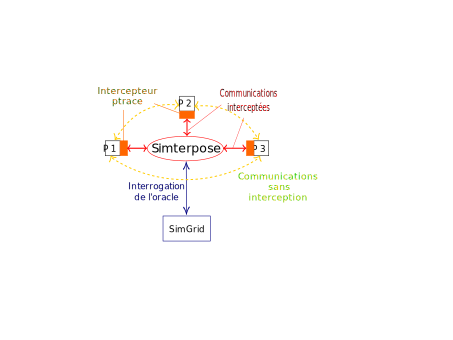
\includegraphics{Pictures/png/Communications_Simterpose_interprocess_v2}
  \caption{Architecture de communications entre les}
  \label{Organisation_generale}
\end{figure}
  
\begin{figure}[H]
  \centering
  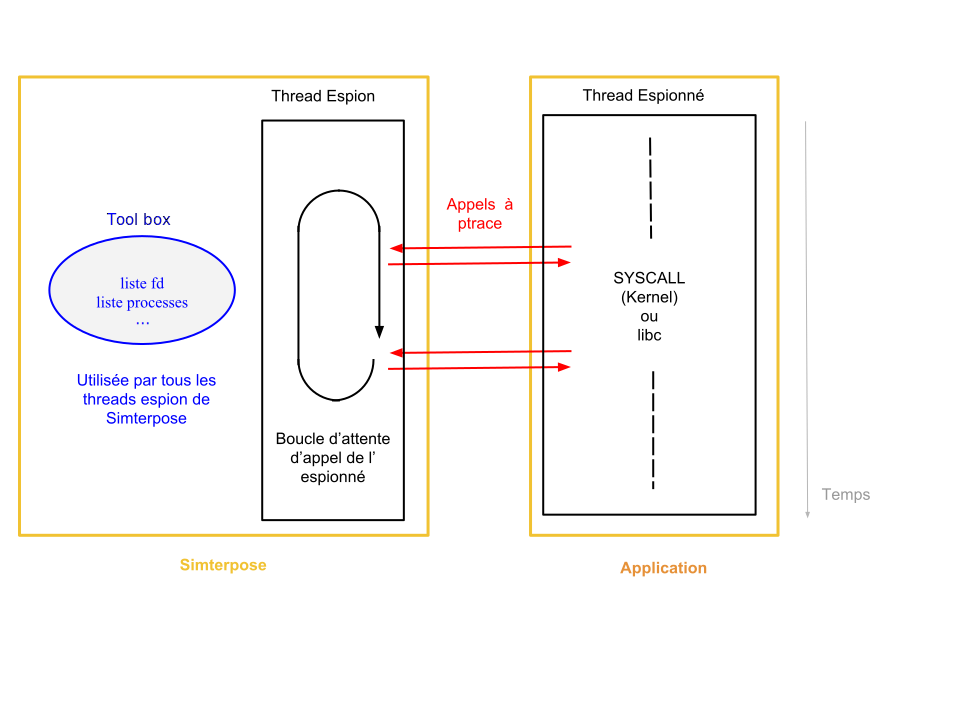
\includegraphics[scale=0.5]{Pictures/png/Simterpose_orga_code_v3}
  \caption{Organisation interne de Simterpose entre un processus espionné et son espion}
  \label{Organisation_Simterpose}
\end{figure}

{\color{red} \textbf{TODO}}

\input{src/4.Simterpose.2.Res.tex}
\subsubsection{Les threads}
 %% syscall clone + libcalls

La gestion des threads se fera à deux niveaux dans Simterpose. On utilise l'interception d'appels système via \texttt{ptrace} pour tout ce qui concerne la création de threads (\texttt{fork}(), \texttt{clone}(), \texttt{pthread\_create}()). Pour le reste on doit utiliser un autre outil, car il existe des mécanismes utilisés par les threads qui ne passent pas par des appels systèmes pour s'exécuter, par exemple les futex\footnote{fast User-space mutex \\ \url{http://man7.org/linux/man-pages/man7/futex.7.html}}. On va donc utiliser le préchargement de bibliothèques dynamiques en complément. Comme nous l'avons vu en section \ref{paragraphe:LDPreload}, nous allons créer une librairie contenant toutes les fonctions utilisées par les threads que nous voulons intercepter (\texttt{pthread\_init}(), \texttt{pthread\_join}(), \texttt{pthread\_exit}(), \texttt{pthread\_yield}() ...). On placera ensuite la bibliothèque dans la variable d'environnement \texttt{LD\_PRELOAD} pour que nos fonctions passent avant les autres.



\subsubsection{Le temps}
 %% -> syscall (- system wide), VDSO-linker (cross process ou VDSO)

Nous souhaitons que l'écoulement du temps perçu par les applications soit un
temps virtuel, celui qui s'écoulerait dans l'environnement virtuel, pour que
l'émulation soit plus réaliste. Il y a deux types d'actions à différencier pour
gérer le temps: les appels de fonctions liées au temps et les actions faites par
l'application qui prenne du temps lors de leur exécution. Dans le premier cas,
Simterpose va intercepter les appels de fonctions temporelles et les modifier
pour renvoyer l'heure virtuelle. Ces dernière étant assez nombreuses, il est
moins coûteux, en terme charge de travail pour l'utilisateur, d'intercepter via
\texttt{ptrace} les appels sytèmes temporels (\texttt{time}(),
\texttt{clock\_gettime}(), \texttt{gettimeofday}()).

Néanmoins, il a été montré dans un précédent stage
\citep{CHLOE:Emulationapplicationdistribuees} que \texttt{ptrace} est inefficace
voire inutile en ce qui concerne l'interception des appels systèmes temporels
qu'une application souhaiterait exécuter car le noyau ne les exécute pas. Cela
est dû à l'existence de la bibliothèque \textit{Virtual Dynamic Shared Object}
(VDSO). Cette dernière vise à minimiser les coûts dûs aux deux changements de
contexte effectués lors de l'exécution d'un appel système. VDSO va retrouver
l'heure dans le contexte noyau lisible par tous les processus sans changer de
mode. Il est possible de désactiver cette bibliothèque lors du boot mais cela
réduit les performances, augmentation du nombre de changements de contexte, et
oblige l'utilisateur à modifier les paramètres de son noyau.

On va donc se placer à un autre niveau pour intercepter ces fonctions. Malgrè
leur nombre il a été décidé d'agir lors du préchargement de bibliothèque. On va
créer une bibliothèque qui surcharge les appels de fonctions liées au temps et
la placer dans la variable d'environnement \texttt{LD\_PRELOAD}, comme nous
l'avons vu en section \ref{paragraphe:LDPreload}. Néanmoins il faut faire
attention de n'oublier aucune fonction.Une fois l'interception temporelle
effectuée, Simterpose interroge SimGrid pour obtenir l'heure virtuelle et la
renvoie à l'application.

Dans le cas d'une action interceptée (calcul, communications réseaux),
Simterpose doit gérer l'horloge de l'application avant de lui renvoyer le
résultat de l'exécution. Pour cela, Simterpose envoie à SimGrid l'heure et la
durée d'exécution sur la machine hôte . Ce dernier calcule en fonction de ces
deux informations, le temps qui aurait été nécessaire pour une telle exécution
sur la plateforme virtuelle et l'envoie à Simterpose. Pour finir, l'émulateur
rend la main à l'application en lui envoyant l'heure virtuelle en plus du
résultat de son action.

\subsection{DNS}
%% libcalls (ne rien rater), config fake (system wide), intercept 53 ( plus dur que nécessaire, port dns autre ou pas)

\input{src/4.Simterpose.6.Ccl.tex}

\newpage
\section{Travail réalisé}
\label{section:work}
Au cours de ce stage, deux des fonctionnalités majeures de Simterpose présentées en section \ref{subsection:fonctionnement_simterpose} ont été implémentées. Il s'agit du réseau de communication et de la gestion du temps. Ces fonctionalités ont parfois nécessité la mise en place de nouvelles fonctionnalités qui n'avaient pas été prise en comptes lors de la création de Simterpose. Dans cette section, nous allons présenter les deux fonctionnalitées implémentées ainsi que les outils qu'elles ont nécessités.

\subsection{Réseau de communications}

\begin{itemize}
\item sys\_file: car on veut des appli distribuées notamment torrent =>gestion fichier
\item deux mediation pour chaque appel paragraph section précédente + description pour chaque appel de ce qu'on fait mettre un exemple de code peut-être
\end{itemize}

\subsection{Temps}
\begin{itemize}
\item paragraph section précédente LD\_PRELOAD
\item pourquoi protéger temps simulation
\item nouvel AS pour gérer le temps dans Simterpose
\item deux mediation pour chaque appel pourquoi non
\end{itemize}

Simgrid + Valgrind + archi 

\subsection{Améliorations apportées à Simterpose}

Lorsqu'on intercepte les appels systèmes il faut pouvoir récupérer les valeurs contenues dans les registre en entrée puis pouvoir écrire dans ces mêmes registres à la sortie de l'appel. Or, au début de mon stage, Simterpose était spécifique aux architectures 64bits. Il ne gérait pas le remplissage des registres et l'utilisation de ces derniers lorsqu'on utilisait une architecture 32bits. Nous avons donc cherché les différences entre ces deux architectures afin de pouvoir exécuter Simterpose sur des plateformes 32bits. La première différence entre ces deux architectures est que les registres ne portent pas les mêmes noms en 64bits et 32bits, cf tableau \ref{register}. Il faut donc utiliser des noms différents selon l'architecture si on veut récuperer des valeurs. Deuxièmement, certaines \texttt{macro} et appels systèmes n'existent pas sur des architectures 64bits et inversement. C'est la cas de deux appels systèmes particulièrement importants car ils touchent au réseau: \texttt{send} et \texttt{recv}. Ces deux appels ne sont définis que pour des architectures 32bits, sur des architectures 64bits quand on les utilise ils sont remplacés par les appels sytèmes \texttt{sendto} et \texttt{recvfrom}.

Ensuite, une mise à niveau de Simterpose a été effectuée afin qu'il puisse utiliser les dernières version de SimGrid. Pour cela il a fallu remplacer de vieilles fonctions encore utilisées dans le code de Simterpose par les nouvelles utilisées dans SimGrid. Cela a également permi de mettre à jour un problème dans SimGrid dû à l'accès d'un pointeur dont on ne vérifiait pas qu'il n'était pas nul. Au début de mon stage, Simterpose utilisait une version de SimGrid datant de 2011, maintenant il utilise la version  {\color{red}XXX} sorti en {\color{red}XXX} 2015.

De plus, nous souhaitions pouvoir utiliser un autre {\color{red}débogueur} en plus de \texttt{gdb}. Nous avons choisi Valgrind pour les nombreux modules qu'il fourni. Notamment \texttt{memcheck} qui est pour nous le plus intéressant. Ce dernier traque les fuites mémoires et résume en fin d'exécution tout ce qui a été réservé, libérée et perdu en mémoire. Pour permettre son utilisation avec Simterpose nous avons dû implémenter l'appel système \texttt{fcntl}. Valgrind utilise cet appel système pour accéder à l'exécution de Simterpose et peut ainsi la controler pour chercher les fuites mémoires. Cela n'était pas prévu à la création de Simterpose puisque nous souhaitons juste intercepter les appels systèmes réseaux, temporels et gérer les processus et leurs threads pour maintenir notre environnement virtuel et aucun  {\color{red}débogueur} autre que \texttt{gdb} ne souhaitait être utilisé à ce moment-là.

Pour finir, le but de Simterpose est d'exécuter des applications distribuées large échelle, notamment des applciations de Torrent. De fait, lorsqu'on exécute des applications de ce type, le système de fichier de la machine hôte est en permanence utilisé. Simterpose dispose en parallèle de son propre système de fihier. Pour chaque socket ou fichier il dispose d'un descripteur avec des compteurs de références, les processus qui les référencent, les verrous qui peuvent être posés... Nous devons donc nous aussi maintenir à jour notre système de fichier dans le cas où nous lancerions ce genre d'applications. Ainsi, nous devons maintenant intercepter les appels systèmes touchant aux fichier en plus de ceux affectant le réseau en utilisant toujours \texttt{ptrace}. Lorsqu'on les intercepte il faut récupérer les modifications qui seront effectués sur le système de fichier réel une fois qu'on aura laisser passer l'appel système et les appliquer au système de fichier propre à Simterpose. Actuellement Simterpose gére les appels systèmes: \texttt{open},  \texttt{close}, \texttt{creat}, \texttt{dup}, \texttt{dup2}, \texttt{poll}, \texttt{fcntl}, \texttt{lseek}, \texttt{read}, \texttt{write}.

\subsection{Réseau de communications}
Pour implémenter le réseau de communications, tel que présenté en section \ref{subsubsection:nework}, nous avons écrit pour chaque appel sysèteme réseaux une version de l'appel utilisant la \textit{médiation par traduction d'adresses} et une utilisant la \textit{full mediation}.

Dans la version de l'appel système utilisant la \textit{médiation par traduction d'adresses}, nous allons récupérer via \texttt{ptrace} les valeurs contenues dans les registres. Ensuite, selon le type d'appel système réseau dont il s'agit on effectue différentes actions sur les paramètres de l'appel. Pour les appels qui concernent l'ouverture et la fermeture de connexion (\texttt{bind}, \texttt{connect}, \texttt{listen}, \texttt{accept}, \texttt{shutdown}, \texttt{close}), ainsi que la création de socket on créé dans la table de correspondance de nouvelles entrées pour permettre de maintenir la virtualisation en traduisant les coupples <IP, port>virtuel en <IP, port>réel si il n'existent pas déjà. Pour les appels concernant les échanges de messages, afin de maintenir notre virtualisation, on cherche les valeurs passées en paramètres de l'appel qui caractérisent le réseau (port, adresse, numéro de socket...). Puis, on récupère en utilisant les tables de traductions <IP, port>virtuel / <IP, port>réel, les valeur réelles correspondantes qui nous intéressent. Pour finir, quelque soit l'appel système, on va écrire les valeurs traduites dans les registres de l'appel système grâce à notre intercepteur \texttt{ptrace} et on laisse l'appel s'exécuter. A la sortie, on refait la même chose à la seule différence qu'on traduit le couple  <IP, port>réel en <IP, port>virtuel.

Pour la version de l'appel système utilisant la \textit{full mediation}, on récupère comme précédement les paramètres de l'appel système contenus dans les registres. On neutralise l'appel système via \texttt{ptrace} pour empêcher son exécution quand on rendra la main à l'application. Puis, selon le type d'appel système réseau dont il s'agit on effectue différentes actions. Pour les appels qui concernent l'ouverture et la fermeture de connexion, ainsi que la création de socket on ne fait rien de particulier puisque dans ce type de médiation aucune socket n'est créée et connectée. Pour les appels systèmes qui correspondent à l'échange de messages on va créer une tâche SimGrid qui va permettre d'écrire ou de lire les données à envoyer ou recevoir. Puis, pour tous les appels systèmes, on va écrire dans les registres de l'appel avec \texttt{ptrace}, la valeur de retour et tout ce qui doit être modifié dans les registres en se basant sur ce que fait réellement l'appel quand il s'exécute réellement. Par exemple, quand on reçoit des données, les données lues dans la tâche SimGrid vont être écrites dans le bufer d'écriture dont l'adresse passée en paramètre est contenue dans un registre.


\subsection{Temps}
\begin{itemize}
\item paragraph section précédente LD\_PRELOAD
\item pourquoi protéger temps simulation
\item nouvel AS pour gérer le temps dans Simterpose
\item deux mediation pour chaque appel pourquoi non
\end{itemize}

\input{src/5.Work.4.Ccl.tex}

\newpage
\section{Évaluation des fonctionalités implémentées}
\label{section:evaluation}
{\color{red} TODO}

\begin{itemize}
\item transition avec section précédente
\item description architecture de tests
\item fonctionnalité implémentée
\end{itemize}

\subsection{Réseaux}
\label{subsection:res}
\subsubsection{Protocole}
\begin{itemize}
  \item Calcul temps simulation
  \item Plateforme reseux ou pas?
\end{itemize}

Dans la section \ref{subsubsection:fonctionnement_reseau}, nous avons présenté l'oganisation du réseau de communications de Simterpose. Après avoir implémenté cette fonctionalité, nous avons souhaité évaluer ses performances à travers divers tests.

L'objectif principal étant de montrer qu'il est possible de faire de la virtualisation légère, nous souhaitons d'abord mesurer l'\textit{overhead} dû à l'utilisation de Simterpose. De cette façon, si le surcoût d'utilisation de notre émulateur est négligeable on pourra conclure que ce type de virtualisation est possible pour le réseau. Dans un second temps, nous souhaitons mesurer les performances des deux types de médiations que nous avons implémentés. Cela nous permettrait de savoir le type de médiation qu'il vaut mieux utiliser selon l'application que l'on souhaite exécuter.

Pour effectuer nos expériences, nous avons utilisé à chaque fois deux applications réseau d'échanges de messages. La première application consiste à faire communiquer un client et un serveur en envoyant au serveur un million de messages de petite taille. La seconde va envoyer depuis un client un message de 1Mo à un serveur. Le protocole pour chaque expérience a été d'exécuter 20 fois chaque application en utilisant les mêmes appels systèmes pour communiquer les messages ({\color{red}sendto/recvfrom et sendmsg/recvmsg}), puis une moyenne du temps d'exécution ainsi qu'une mesure des temps minimum et maximum ont été conservées.

\subsubsection{Overhead conçernant le temps d'exécution}
Afin de mesurer l'\textit{overhead} produit par Simterpose, nous avons exécutés les deux applications réseaux présentées plus haut sur une machine en utilisant uniquement le réseau local puis en utilisant Simterpose. Ainsi, en comparant les temps d'exécution des applications sur les deux types d'architecture nous pourrons calculer l'\textit{overhead}. Les résultats de ces expériences sont présentés Figures \ref{Network_Big_Local} et \ref{Network_Little_Local}.

Dans le cas de l'envoi de plusieurs petits messages le temps moyens d'exécution en local est d'environ 3 secondes, avec Simterpose on arrive à 72 secondes en \textit{full mediation} et à 75 secondes en \textit{médiation par traduction d'adresse}. On a donc une exécution qui prend 25 fois plus de temps. De même, lors de l'envoi d'un gros message le système met 0,01 secondes en moyenne pour exécuter l'application alors que Simterpose met entre 1 et 1,1 secondes selon le type de médiation. Cette exécution prendra donc 100 fois plus de temps si on souhaite réellement mettre en place notre émulateur.

\begin{figure}
  \centering
    \includegraphics[scale=0.5]{mesures/graph/Bigmsg_local.jpg}
    \caption{Temps d'exécution lors de l'envoi d'un message de 1Mo avec et sans Simterpose.}
    \label{Network_Big_Local}
\end{figure}

\begin{figure}
  \centering
    \includegraphics[scale=0.5]{mesures/graph/Littlemsg_local.jpg}
    \caption{Temps d'exécution lors de l'envoi d'un million de messages de 128o avec et sans Simterpose.}
    \label{Network_Little_Local}
\end{figure}
  
Néanmoins, cet écart s'explique par les nombreux appels systèmes et changements de contexte que nécessite Simterpose de par son utilisation coûteuse de ptrace en plus de l'exécution de l'appel système lui-même (lorsqu'on utilise \textit{médiation par traduction d'adresse}). Pour la première expérience on peut considérer que cet \textit{overhead} représente un cas extrême car les utilisateurs en général ne testent pas leurs applications en envoyant des millions de message entre un client et un serveur. De plus, du point de vue humain une exécution de 1ms ou 1s dans le second cas ne change pas grand chose pour notre perception. Ainsi, on peut considérer que l'\textit{overhead} produit par Simterpose sur le temps d'exécution est acceptable.

\subsubsection{Quelle médiation pour quel type d'application}
 Pour comparer les deux médiations que nous avons implémentés, nous avons utilisé le protocole présenté précédement. Les résultats de notre expérience sont présentés Figures \ref{Network_Big_Mediation} et \ref{Network_Little_Mediation}.

Lorsque l'on envoie de nombreux petits messages, on peut constater que la \textit{full mediation} est plus rapide que la \textit{médiation par traduction d'adresse} avec un écart moyen de 3 secondes. Ce résultat s'explique par le fait que lorsqu'on utilise la \textit{médiation par traduction d'adresse} l'envoi de messages génère des appels systèmes et changements de contexte qui n'ont pas lieu en \textit{full mediation} puisque dans ce cas, comme nous l'avons expliqué en section \ref{paragraph:FULL_MEDIATION}, les appels systèmes ne sont pas exécutés. Ces derniers étant couteux cela explique pourquoi la  \textit{médiation par traduction d'adresse} est moins rapide. De plus, en \textit{full mediation}, même si les appels systèmes sont bloqués, nous utilisons l'appel système ptrace pour effectuer nous-même les appels demandés par l'application que nous avons bloqués. Cette méthode même si elle reste moins couteuse que l'exécution de l'appel système demandé consomme des cycles CPU, ce qui explique le faible écart entre les temps d'exécution moyen des deux types de médiation.

Lorsque l'on envoie un gros message, on constate que l'écart moyen entre les deux types de médiation est quasi nul, 0.03 secondes. Nous pensons que dans ce cas la \textit{médiation par traduction d'adresse} est légèrement plus rapide car nous envoyons un seul message de 1Mo de données. En effet, même en \textit{full mediation} on a beaucoup moins de changement de contexte de par le blocage des appels systèmes ici on ne fait qu'un seul appel et la faible différence entre les deux médiations ne peut donc être dû à cela. Par contre, lors de l'envoi d'un tel message il faut prendre en compte la gestion de la mémoire car le message doit être stocké avant de pouvoir être envoyé par morceau sur le réseau. Ainsi, si on ne gère pas la mémoire de façon efficace on surconsomme des cycles CPU. Or, nous n'avons pas encore mis en place de politique de gestion de mémoire particulière pour Simterpose. Néanmoins, si on regarde la largueur des intervalles des temps d'exécution, en \textit{médiation par traduction d'adresse} les temps d'exécution varient bien plus qu'en \textit{full mediation}. On peut donc supposer qu'avec une politique de gestion mémoire aussi efficace que celle qui est utilisée par le système la \textit{full mediation} serait probablement plus rapide que la \textit{médiation par traduction d'adresse} comme dans l'expérience précédente.

\begin{figure}
  \centering
    \includegraphics[scale=0.5]{mesures/graph/Bigmsg.jpg}
    \caption{Temps d'exécution lors de l'envoi d'un message de 1Mo avec et sans Simterpose.}
    \label{Network_Big_Mediation}
\end{figure}

\begin{figure}
  \centering
    \includegraphics[scale=0.5]{mesures/graph/Littlemsg.jpg}
    \caption{Temps d'exécution de l'envoi d'un million de messages de 128o avec et sans Simterpose.}
    \label{Network_Little_Mediation}
\end{figure}

Ces expériences nous ont permis de montrer que lors de l'envoi de nombreux messages il vaut mieux privilégier la \textit{full mediation}. Nous avons également pu voir que pour envoyer de gros messages, les deux médiations se valent. De plus, la faible durée d'exécution d'une expérience nous permet de considérer que l'overhead dû à la mise en place de Simterpose est acceptable. Ainsi, nous pouvons dire que notre implémentation du réseau de communications permet de faire de la virtualisation légère à ce niveau. Nous allons maintenant voir si il en est de même en ce qui concerne la gestion du temps.

\subsection{Temps}
\label{section:temps}
Dans la section, nous avons pu voir qu'il est important de gérer le temps que l'applciation voit s'écouler. En section , nous avons présenté l'implémentation qui a été choisie pour résoudre cette problématique. Maintenant, nous souhaitons mesurer le surcoût ajouté par cette fonctionnalité lors de l'exécution de Simterpose. Si ce surcoût est acceptable, on pourra considérer qu'il est également possible de mettre en place une virtualisation légère qui gère l'écoulement du temps.

\subsubsection{Protocole}
Pour évaluer notre implémentation nous n'allons pas utiliser les mêmes expériences que pour le réseau de communications car le but ici est d'intercepter de les fonctions temporelles et mesurer le coût de cette interception. Ainsi, nous avons créé une application qui exécute différents appels à des fonctions temporelles (ftime, time, gettimeofday, localtime, mktime...). Le protocole utilisé pour exécuter l'application est également différent. Nos expériences vont ici consister à exécuter 20 fois l'application dans quatre configurations différentes qui soient comparables. Tout d'abord nous allons exécuter l'application qui effectue les appels temporels avec Simterpose en \textit{full mediation} sans LD\_PRELOAD, puis avec LD\_PRELOAD. Puis nous ferons de même pour la \textit{médiation par traduction d'adresse}.  Les résultats de ces deux expériences sont présentés Figure \ref{Temps_FM} et \ref{Temps_AT}.

Le changement de médiation ne devrait pas influer sur les performances car elles ne sont appelées que lorsqu'on souhaite effectuer des appels systèmes réseaux que l'on fasse de l'interception avec LD\_PRELOAD ou pas. En comparant les deux graphiques, on voit bien que les courbes d'interception via LD\_PRELOAd se superposent et qu'il en est de même pour celle sans interception malgré la différence de médiation. Cela confirme bien l'hypothèse que nous avons fait. Nous pouvons maintenant nous intéresser à l'impact de l'interception sur chaque médiation.

\subsubsection{Full mediation}
Nous allons d'abord regarder les deux premières expériences: Simterpose en \textit{full mediation} avec et sans intercpetion via LD\_PRELOAD. On constate que le temps d'exécution avec interception via LD\_PRELOAD est plus ou moins constant (environ 1,03 secondes), alors que celui sans interception varie énormément, entre 0,82 et 1,13 secondes. Cela est du au fait que lors d'appel à des fonctions temporels sans interception via LD\_PRELOAD la bibliothèque VDSO, citée en section, est appelée pour gérer l'appel et accéder elle-même à la mémoire. Cette accès n'a pas un coût constant puisqu'il dépend de la charge du système qui varie en permanence même si on ne fait tourner que notre application et aucune autre en parallèle. Ainsi, le temps d'exécution peut varier comme c'est la cas ici alors qu'il est stable quand on utilise LD\_PRELOAD puisqu'on empèche ces accès. Néanmoins, en moyenne les deux expériences ont environ le même temps d'exécution 1 seconde pour la première et 1,02 secondes pour la deuxième. On peut donc considérer que l'interception via LD\_PRELOAD a un surcoût négligeable lorsqu'on utilise Simterpose en \textit{full mediation}.

\begin{figure}
  \centering
    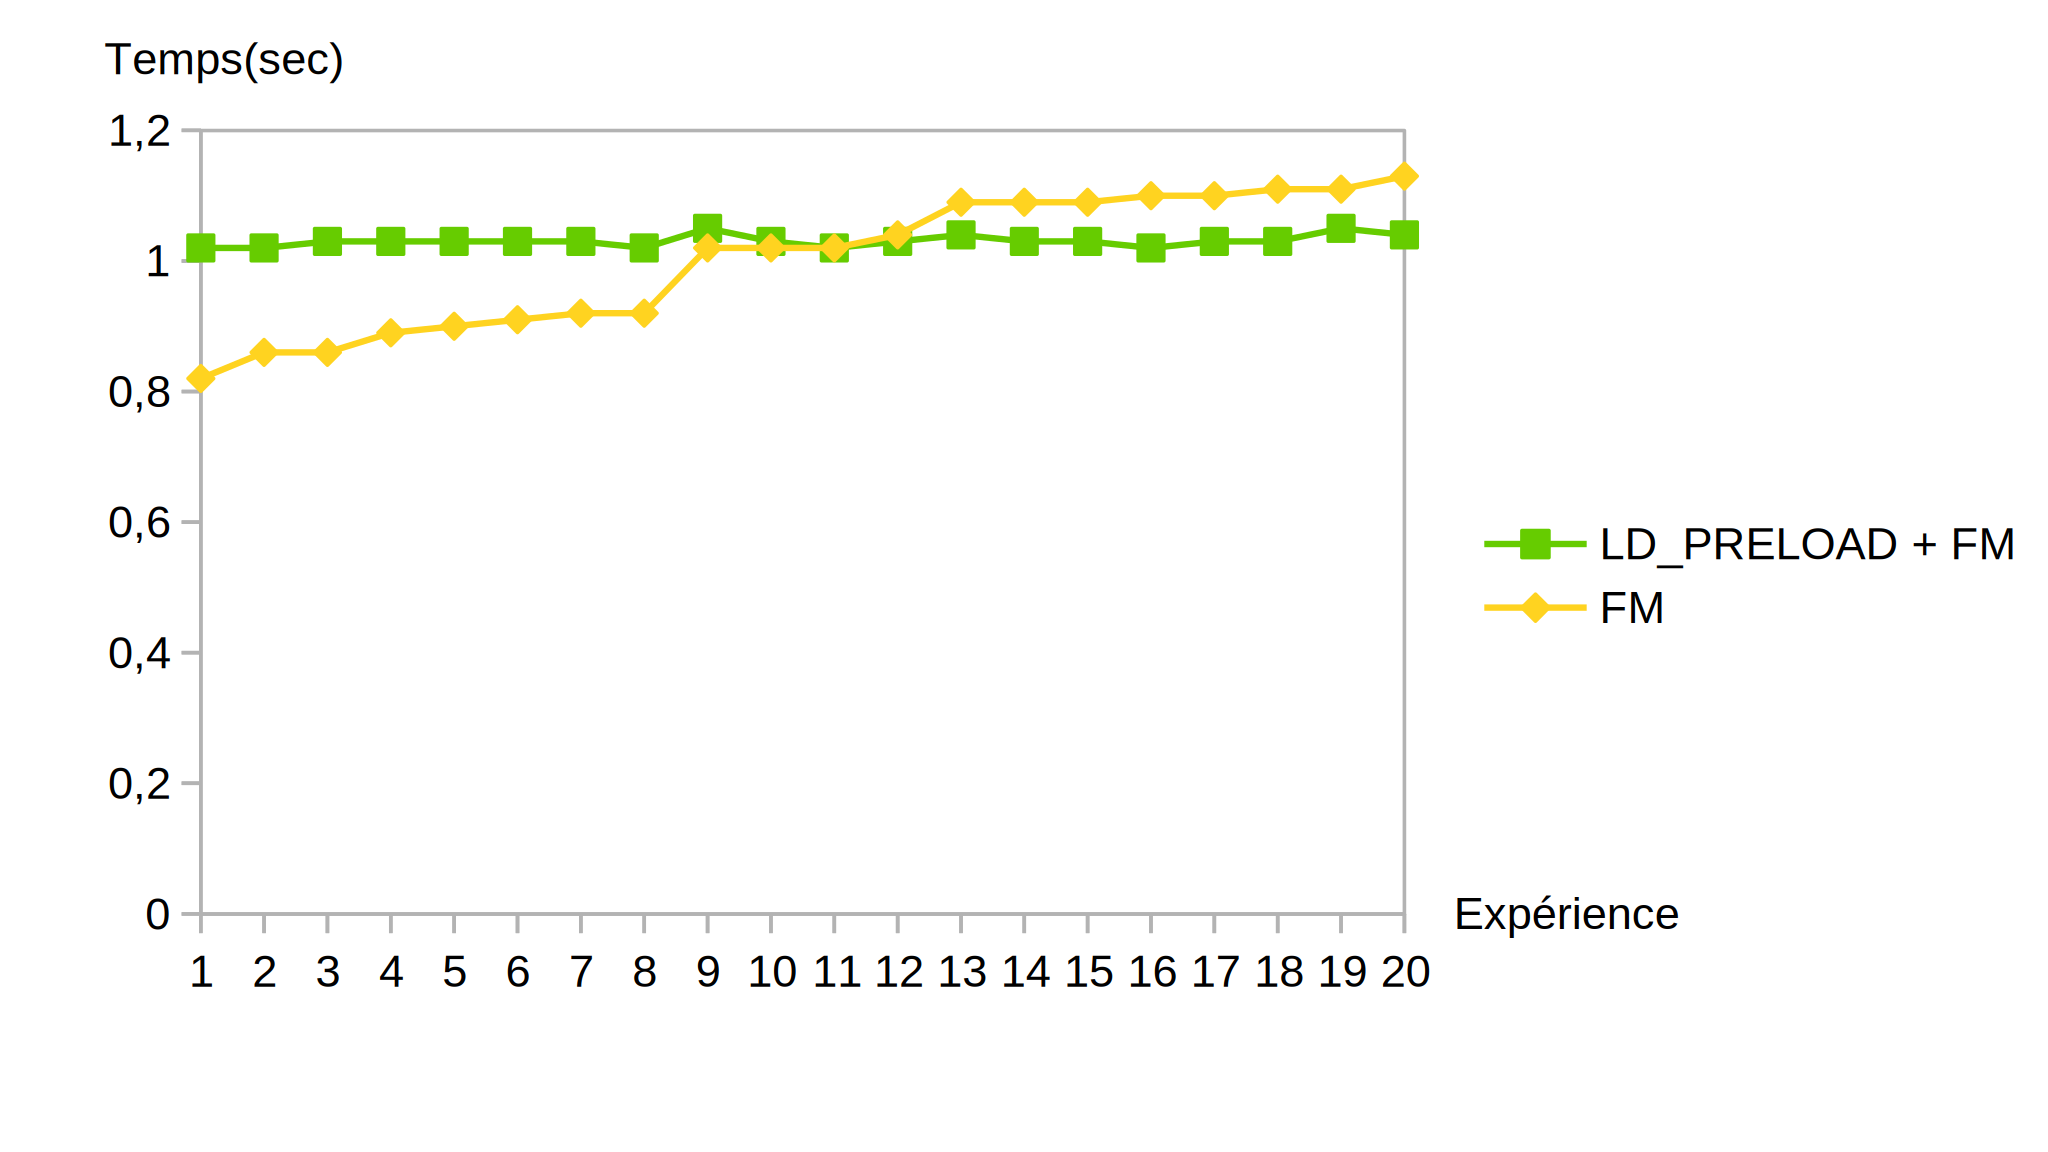
\includegraphics[scale=0.80]{mesures/graph/Temps_FM.png}
    \caption{Temps d'exécution d'une application temporelle en \textit{mediation par traduction d'adresse} avec interception via LD\_PRELOAD et sans interception}
    \label{Temps_FM}
\end{figure}

\subsubsection{Mediation par traduction d'adresse}
Nous allons maintenant voir s'il en est de même pour les deux dernières expériences: Simterpose en \textit{médiation par traduction d'adresse} avec et sans intercpetion via LD\_PRELOAD. On constate ici aussi que le temps d'exécution avec interception via LD\_PRELOAD est plus ou moins constant (environ 1,02 seconde), alors que celui sans interception varie énormément, entre 0,86 et 1,12 secondes. Cela est dû comme précédement à l'utilisation de la bibliothèque VDSO en l'absence d'interception via LD\_PRELOAD. De plus, ici aussi le temps moyen des deux expériences est le même: 1,02 secondes. Dans ce cas, l'interceprtion via LD\_PRELOAD n'a aucun surcoût.

\begin{figure}
  \centering
    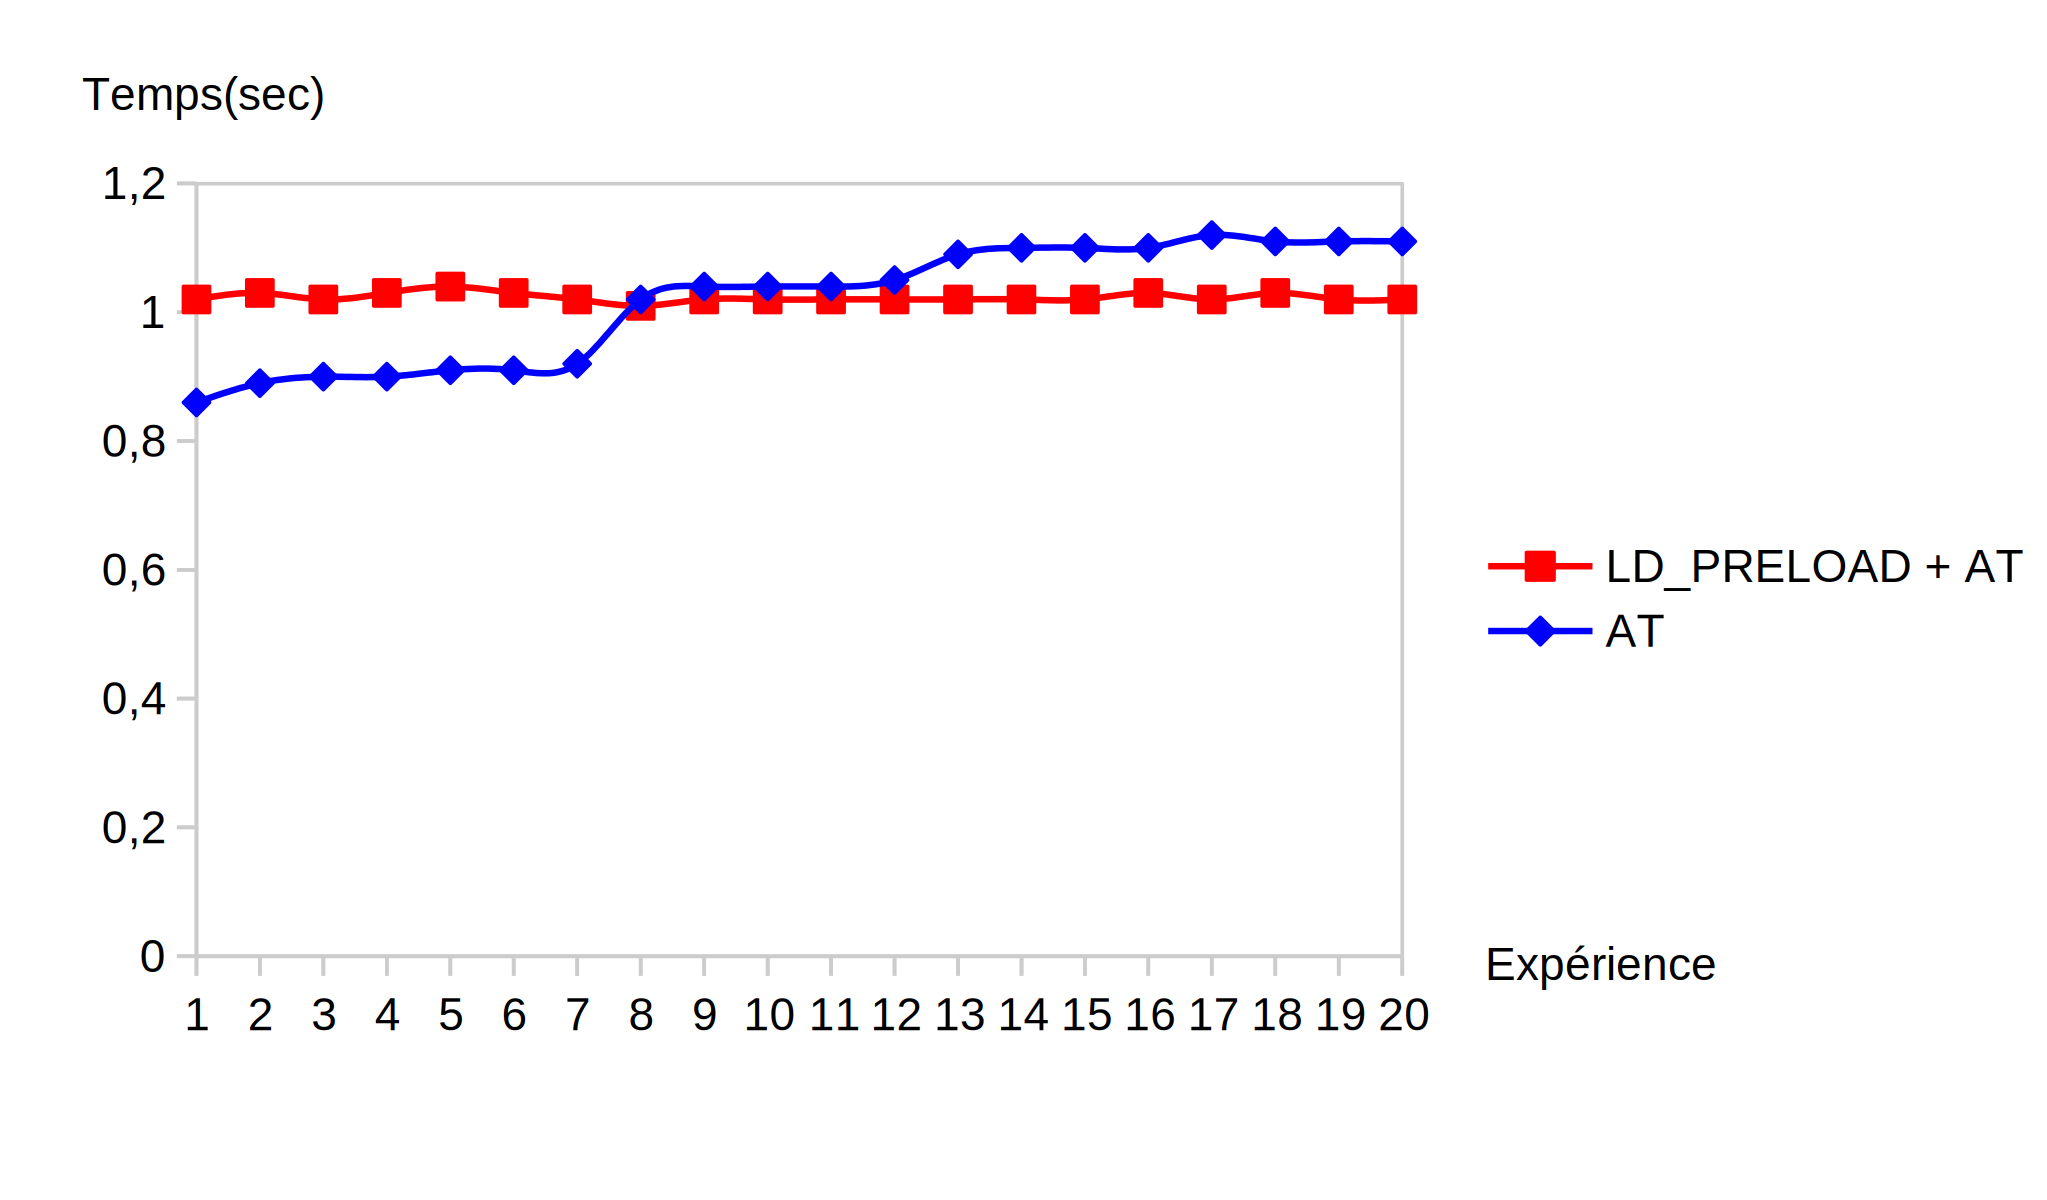
\includegraphics[scale=0.65]{mesures/graph/Temps_AT.jpg}
    \caption{Temps d'exécution d'une application temporelle en \textit{full mediation} avec interception via LD\_PRELOAD et sans interception}
    \label{Temps_AT}
\end{figure}

Ainsi, nous avons pu voir que le surcoût dû à l'interception des fonctions temporelles via LD\_PRELOAD est inexistant en \textit{médiation par traduction d'adresse} et qu'il est négligeable \textit{full mediation} (environ 2\%). On peut donc considérer que nous avons réussi à mettre en place une virtualisation légère qui gère également l'écoulement du temps et qui plus est de façon particulièrement efficace.

\vspace{0.5cm}

\input{src/6.Evaluation.3.Ccl.tex}

\newpage
\input{src/7.Conclusion.tex}

\newpage

% Bib
\bibliographystyle{plainnat}
\bibliography{src/8.Biblio} % The file containing the bibliography
\label{fin}

\end{document}
